\documentclass[a4j]{jarticle}
\usepackage[dvipdfmx]{graphicx}
\usepackage{amssymb}
\usepackage{amsmath}
\usepackage{subfigure}

\setlength\floatsep{0.2pt}
\setlength\abovecaptionskip{0.2pt}

\newcommand{\argmax}{\mathop{\rm arg~max}\limits}

\begin{document}
\begin{table}[t]
\begin{center}
{\large 産業用モニタリングシステムにおける障害検知手法の提案}\\
令和 2 年 9 月 11 日\\
山本 航平
\end{center}
\end{table}

進捗報告
\begin{itemize}
\item のこぎり波の生成モデルの作成に取り組んでいます.
\item 頂いた SIM を用いた計測データを分析しました.
\item FTP を併用した計測データを分析しました.
\end{itemize}

\section{のこぎり波}
一日を通した計測結果の一部を図 \ref{rise} に示す.
この図は横軸を時刻とし,縦軸に対応する時刻に計測した ping 応答値をとった折れ線グラフである.
ただし赤色破線は LTE 接続が切れた時刻を表すが,ここでは取り扱わないので詳細は省く.
この図のように低遅延帯に分布する応答遅延が緩やかに増加していき,しばらくすると急激に減少して再度緩やかに増加していく傾向がみられる.
\begin{figure}[tb]
\begin{center}
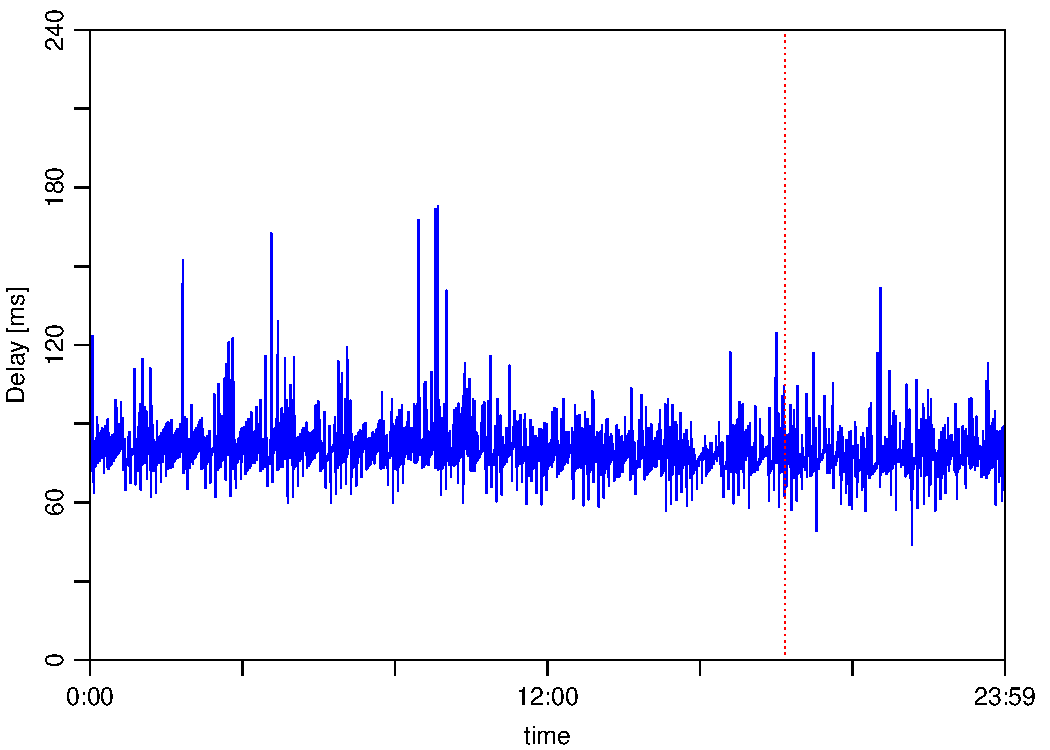
\includegraphics[width=0.8\hsize]{C:/master/mstudy/analysis/long/plot-6-23.pdf}
\caption{6 月 23 日(火)に得られた応答遅延の時間データ}
\label{rise}
\end{center}
\end{figure}
この右肩上がりの傾向は計測日に問わず見られることから,応答遅延の変動の仕方を特徴づけるものと考えられる.

産業用モニタリングシステムにおける障害検知手法の開発に向けて,通常とは異なる遅延変動を通常時のものと切り分け検知するために,通常時の応答遅延の時間データをモデル化することに取り組んだ.
モデル化することで例えば,実環境でリアルタイムに得られる計測値とモデルでの予測値を逐次比較して検知したり,モデルパラメータを計測日時特有もしくは共通した特徴量とみなし,実環境でリアルタイムに計測データのモデル化を行いこの特徴量を比較して検知したりする手法が可能ではないかと考えた.

\section{計測データの前処理}
計測データは図 \ref{rise} のように短期的な変動が激しく特に突発的に特出して大きなまたは小さな応答遅延が発生するため,こののこぎり型の波形の抽出が困難である.
そこで計測データに対してローパスフィルタを用いて短期的な変動を生じさせる高周波数帯を除去し,逆フーリエ変換を行い復元した波形からのこぎり波の抽出を行う.

6 月 23 日の計測データに対してこの前処理を行い,計測時刻が 0 時から 6 時までの一部の波形を図 \ref{lowpass} に示す.
ただし,横軸は計測時刻が早いものから順に 0,1,$\ldots$ としたインデックスを取り,縦軸には応答遅延の値を取っている.
また,青色線が計測値を,赤色線が前処理後の波形を表す.
\begin{figure}[tb]
\begin{center}
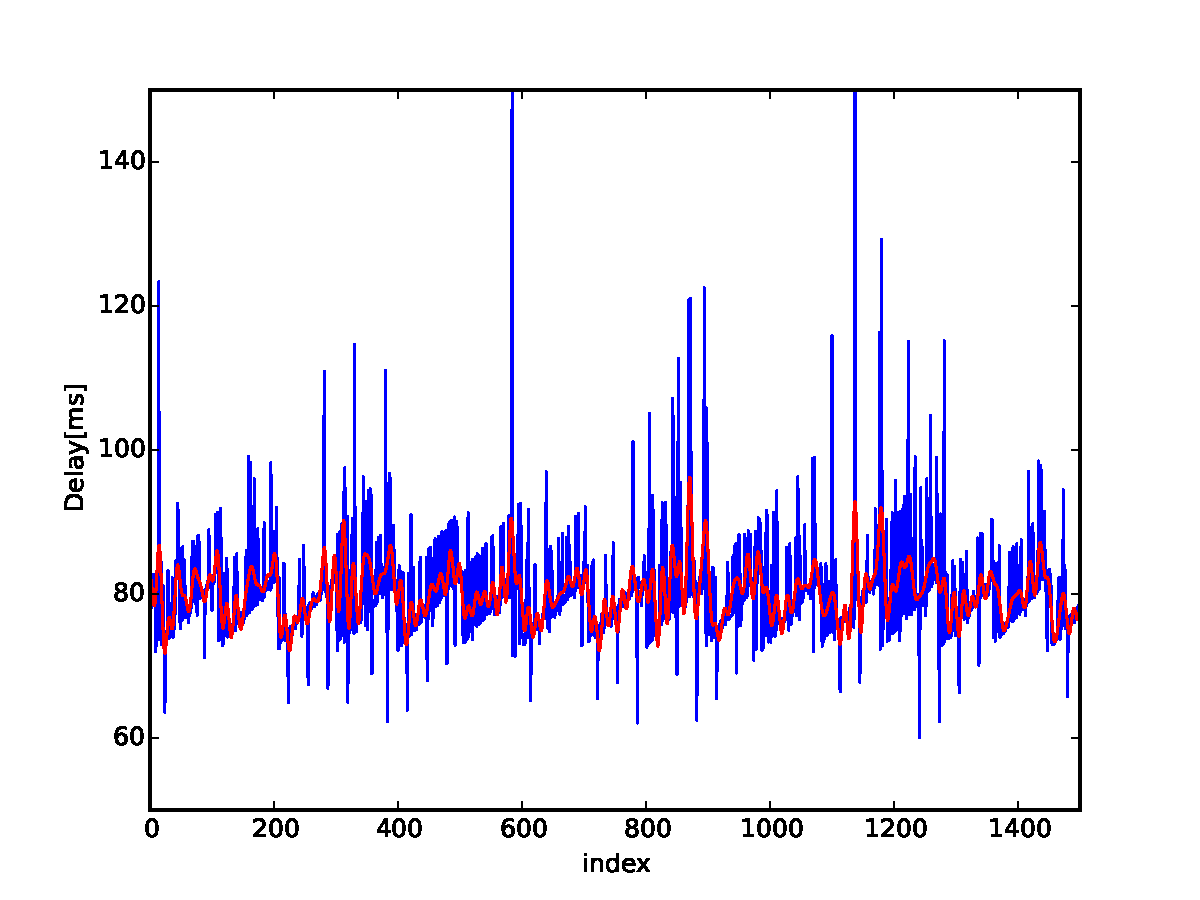
\includegraphics[width=0.8\hsize]{C:/master/mstudy/analysis/0829/lowpass08.pdf}
\caption{計測波形(青線)から 0.008 Hz 以上の波を除去した波形(赤線)}
\label{lowpass}
\end{center}
\end{figure}
ローパスフィルタの値はもと波形の突発的な応答遅延を除去し,かつのこぎり型の波形の各両端が滑らかになりすぎないようになるものが好ましい.
計測波形から定量的にこの値を決めることが望ましいが,ここでは図 \ref{lowpass} の結果からこの値を 0.008 Hz として話を進めることとする.

\section{逐次的な単回帰}
のこぎり波は右肩上がりの直線に見えるので,前処理後の波形に含まれる各のこぎり波は直線で回帰することができ,その回帰結果からのこぎり波を抽出できないかを検討した.

\subsubsection{アルゴリズム}
波形を右肩上がりの直線で回帰できる区間に分割する.
しかし,全区間を一度に分割することは分割数が未知であるため困難である.
そこで,先頭からインデックス幅 200 (計測時間 50 分相当)に含まれる波形を二つに分割したとき前後それぞれの波形を最も精度良く右肩上がりの直線で回帰できる分割点を求め,次はその分割点からさらにインデックス幅 200 までの波形に対して同様の操作により分割点を求める.
この操作を繰り返すことで全体を分割する.
また,このインデックス幅 200 は計測時間 50 分相当であり,6 月 23 日の全区間の計測データに対して FFT を行った結果である図 \ref{fft} からのこぎり型の波形の周期が大体 25 分程度(約 0.0006 Hz)であることをもとに,のこぎり型波形が 2 つよりも多く含まれないように定めた.
\begin{figure}[tb]
\begin{center}
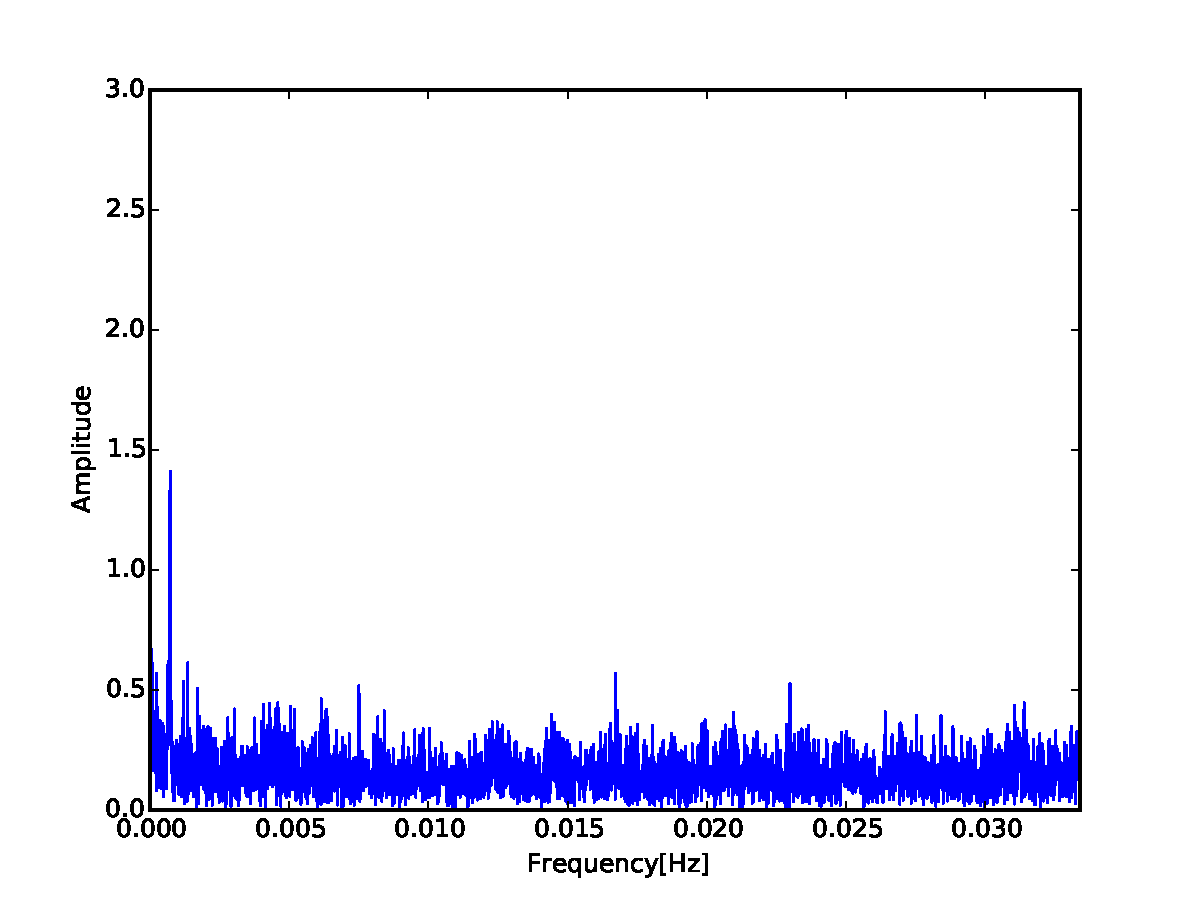
\includegraphics[width=0.8\hsize]{C:/master/mstudy/analysis/0829/fft_6-23.pdf}
\caption{6 月 23 (火)の全区間データに対する FFT (横軸 : 周波数,縦軸 : 振幅)}
\label{fft}
\end{center}
\end{figure}

単回帰には最小二乗法を用い,回帰精度の指標として決定係数の積を用いた.
分割点はインデックス幅 200 の区間で前後二つの回帰線の傾きが共に正かつ指標の値を最大とする時点とする.
また,各回帰線は少なくとも 20 点(約 5 分相当)以上の計測点を回帰するものとする.
表 \ref{alg1} にこの分割方法の疑似コードを示す.\\
\begin{table}[tb]
\caption{逐次的単回帰のアルゴリズム}
\label{alg1}
\begin{tabular}{l}
\hline
$Data$ = (前処理後のデータ列)\\
$C$ = [0] \hspace{1cm}\#分割点のリスト\\
\\
while(1)\{\\
\hspace{0.5cm}for ($20 \leq i \leq 180$)\{\\
\hspace{1cm}$left = C[末尾]$\\
\hspace{1cm}$mid = C[末尾] + i$\\
\hspace{1cm}$right = C[末尾] + 200$\\
\\
\hspace{1cm}$X_1 = 区間 [left, mid)$\\
\hspace{1cm}$Y_1 = Data[X_1]$\\
\\
\hspace{1cm}$X_2 = 区間 [mid, right]$\\
\hspace{1cm}$Y_2 = Data[X_2]$\\
\\
\hspace{1cm}$\widehat{Y_1} = a_1\widehat{X_1} + b_1 \leftarrow 最小二乗法(X_1,Y_1)$\\
\hspace{1cm}$\widehat{Y_2} = a_2\widehat{X_2} + b_2 \leftarrow 最小二乗法(X_2,Y_2)$\\
\hspace{0.5cm}\}\\
\\
\hspace{0.5cm}if($a_1>0$ and $a_2>0$)\\
\hspace{1cm}$C = C \cup \argmax_{20\leq mid \leq 180} \left[1-\frac{\sum \left(Y_1 - \widehat{Y_1}\right)^2}{\sum \left(Y_1 - \overline{Y_1}\right)^2} \right] * \left[1-\frac{\sum \left(Y_2 - \widehat{Y_2}\right)^2}{\sum \left(Y_2 - \overline{Y_2}\right)^2} \right]$\hspace{1cm}$\#\overline{Y}$ は $Y$ の平均値\\
\\
\hspace{0.5cm}if($mid + 200 > データ数)$\hspace{1cm}break\\
\}
\end{tabular}
\end{table}

\subsubsection{実行結果}
実行結果を図 \ref{resultalg1} に示す.
この図は黒線が前処理後の波形を示しており,色線は分割点で分割された各区間の波形の回帰直線である.
これらはともに図の左側を縦軸としている.
また,右側の縦軸には評価値を取っており,アルゴリズム実行中において各色の回帰直線の終了時点に当たる分割点を求める際の評価値を回帰直線と同色の曲線で示した.
\begin{figure}[tb]
\begin{center}
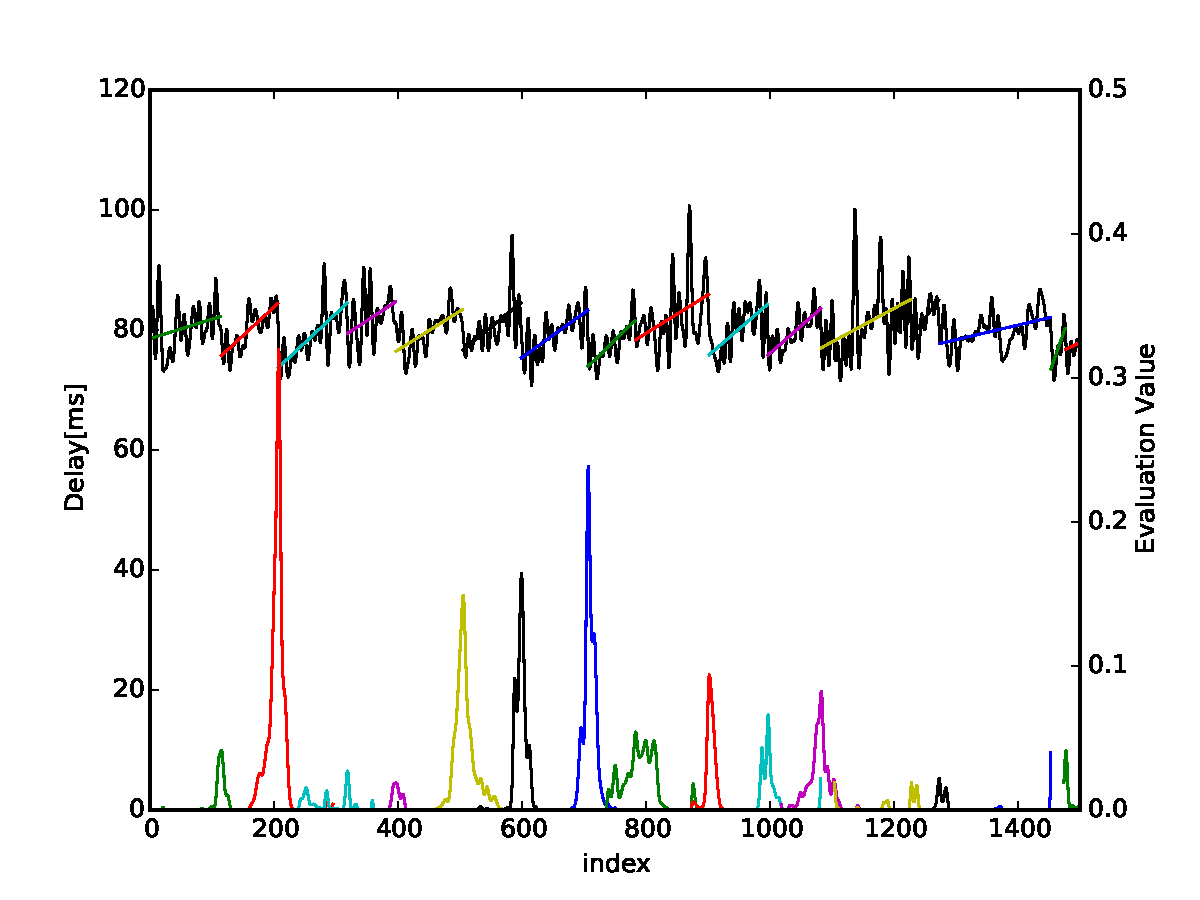
\includegraphics[width=0.8\hsize]{C:/master/mstudy/analysis/0829/resultalg1.pdf}
\caption{手法 1 の実行結果と評価値}
\label{resultalg1}
\end{center}
\end{figure}

図より,おおよそ期待通りの分割がなされており,またこの評価値による分割点の感度は高いことが見て取れる.しかしながら一方で,インデックス 1300 から 1400 の区間では 1350 付近での分割が期待されるがなされていない.これは,最小二乗法による単回帰では回帰線と計測値の誤差を小さくするが,回帰線と計測値の大小関係は考慮していないことから,のこぎり波の両端を示す急激な下振れを検出できなかったと考えられる.
また,インデックス 1100 から 1300 までの区間のように評価値に明確な極大値が存在しないこともあるようだ.

\subsection{エラー対策}
このアルゴリズムはインデックス幅 200 の範囲にはのこぎり波が二つ含まれており,そのそれぞれが傾きが正の直線で回帰できることを想定している.
先の実行結果を見るに多くの場合では期待通りの分割点を抽出できているが,応答遅延の大きさやばらつき具合の影響で傾きが正の直線二つで回帰できない場合がある.そこでこのような場合に限っては,直前の分割点以降の波形を傾き正の直線一本で回帰した場合に決定係数が最大となる時点を次の分割点とした.
\section{計測データの分析}
6 月 23 日から 7 月 22 日までに得られた一日単位の計測データに対してこの手法を用い,のこぎり波を抽出した.
またこの計測データの横軸は計測時刻が早いものから順に 0,1,$\ldots$ と割り当てたインデックスであり,幅 1 あたり 15 秒相当である.
縦軸は応答遅延 [ms] である.

\subsection{のこぎり波の幅}
全計測データののこぎり波の幅の分布は図 \ref{dist-leng} となった.
ビン幅は 2 とした.
\begin{figure}[tb]
\begin{center}
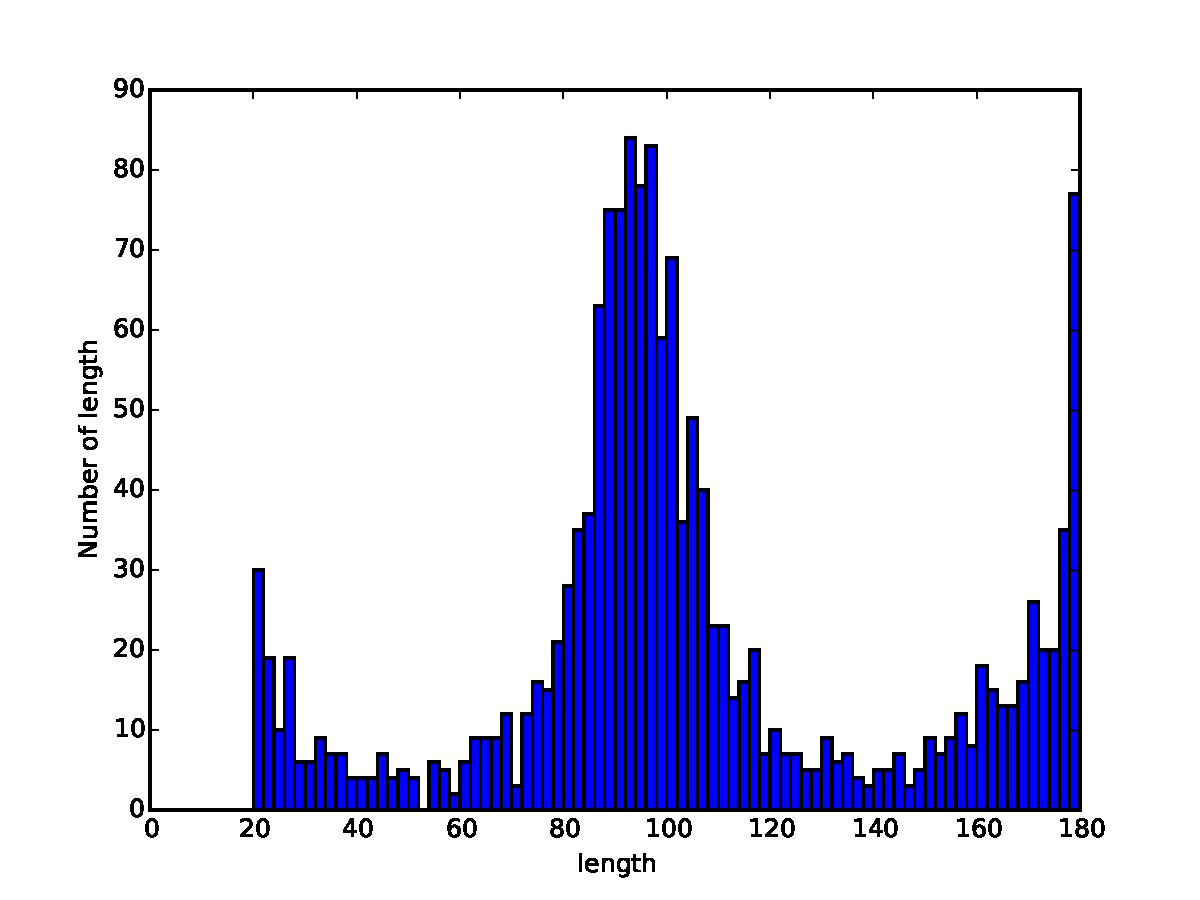
\includegraphics[width=0.8\hsize]{C:/master/mstudy/analysis/model/B_hist_all.pdf}
\caption{のこぎり波の幅の分布}
\label{dist-leng}
\end{center}
\end{figure}
図 \ref{dist-leng} は平均 90 程度の正規分布に見える.
ただし,裾の部分の度数は大きくなっていた.
これは,突発的に発生する大きなもしくは小さな応答遅延や分散が大きい区間の影響により,明確な分割点が存在しなかった場合と考えられる.

また,自己相関は図 \ref{autoCorr-leng} となった.
ここではのこぎり波の幅によらず隣り合うのこぎり波のラグを 1 としている.
青色の範囲はのこぎり波の幅にホワイトノイズが加わることを仮定した場合の信頼区間 95 \% の範囲であるが,用いたパッケージの影響で描写されたものでありここでは特に意味をなさない.
\begin{figure}[tb]
\begin{center}
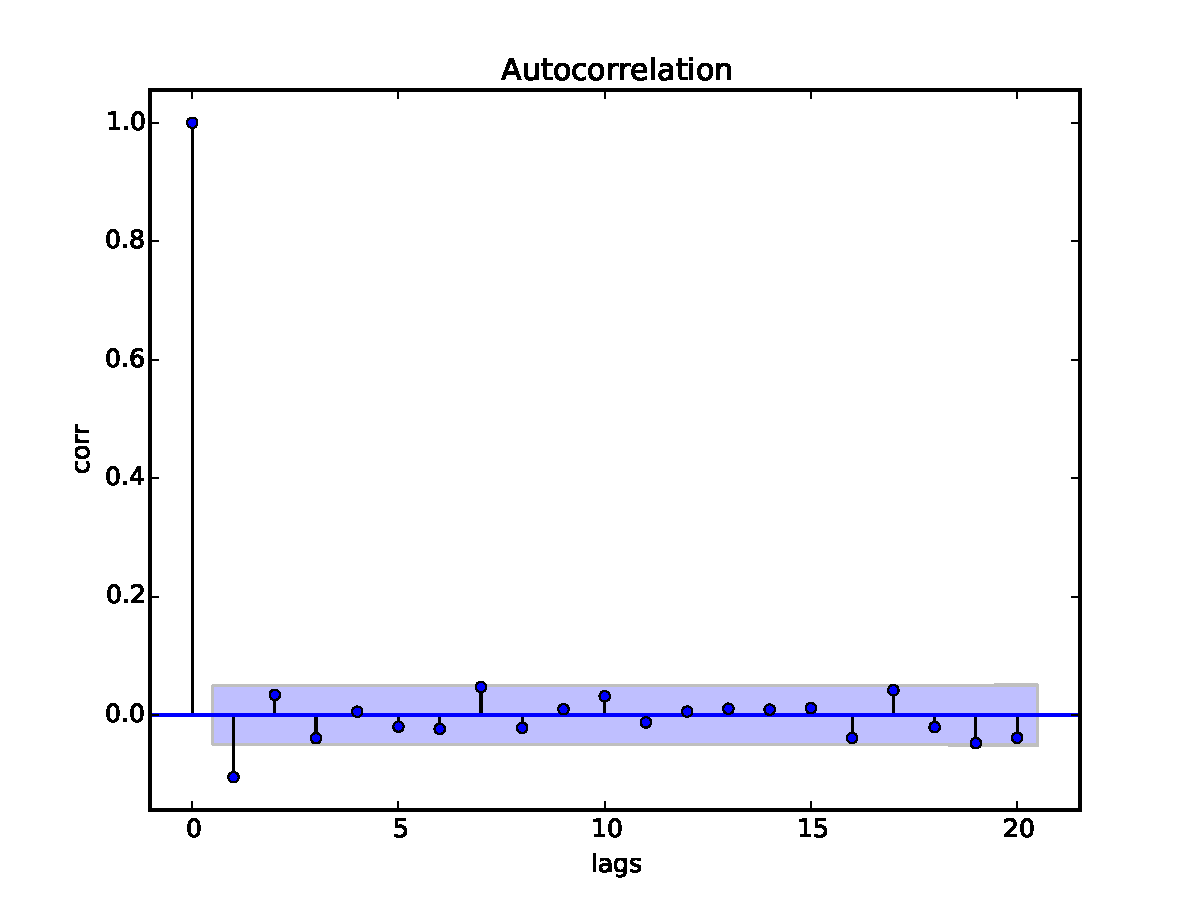
\includegraphics[width=0.8\hsize]{C:/master/mstudy/analysis/model/autoCorr-B.pdf}
\caption{のこぎり波の幅の自己相関}
\label{autoCorr-leng}
\end{center}
\end{figure}
図 \ref{autoCorr-leng} より,あるのこぎり波とその直後 20 個ののこぎり波の幅には相関は見られず,独立であると考えられる.

加えて,平均値と分散を表 \ref{stat-leng} に示す.
\begin{table}[tb]
\begin{center}
\caption{のこぎり波の幅の統計量}
\label{stat-leng}
\begin{tabular}{|c|c|}
\hline
平均(少数第二位以下四捨五入)&分散(少数第二位以下四捨五入)\\
\hline
103.9&1585.4\\
\hline
\end{tabular}
\end{center}
\end{table}

\subsection{のこぎり波の傾き}
全計測データののこぎり波の傾きの分布は図 \ref{dist-inc} となった.
ビン幅は 0.01 とした.
\begin{figure}[tb]
\begin{center}
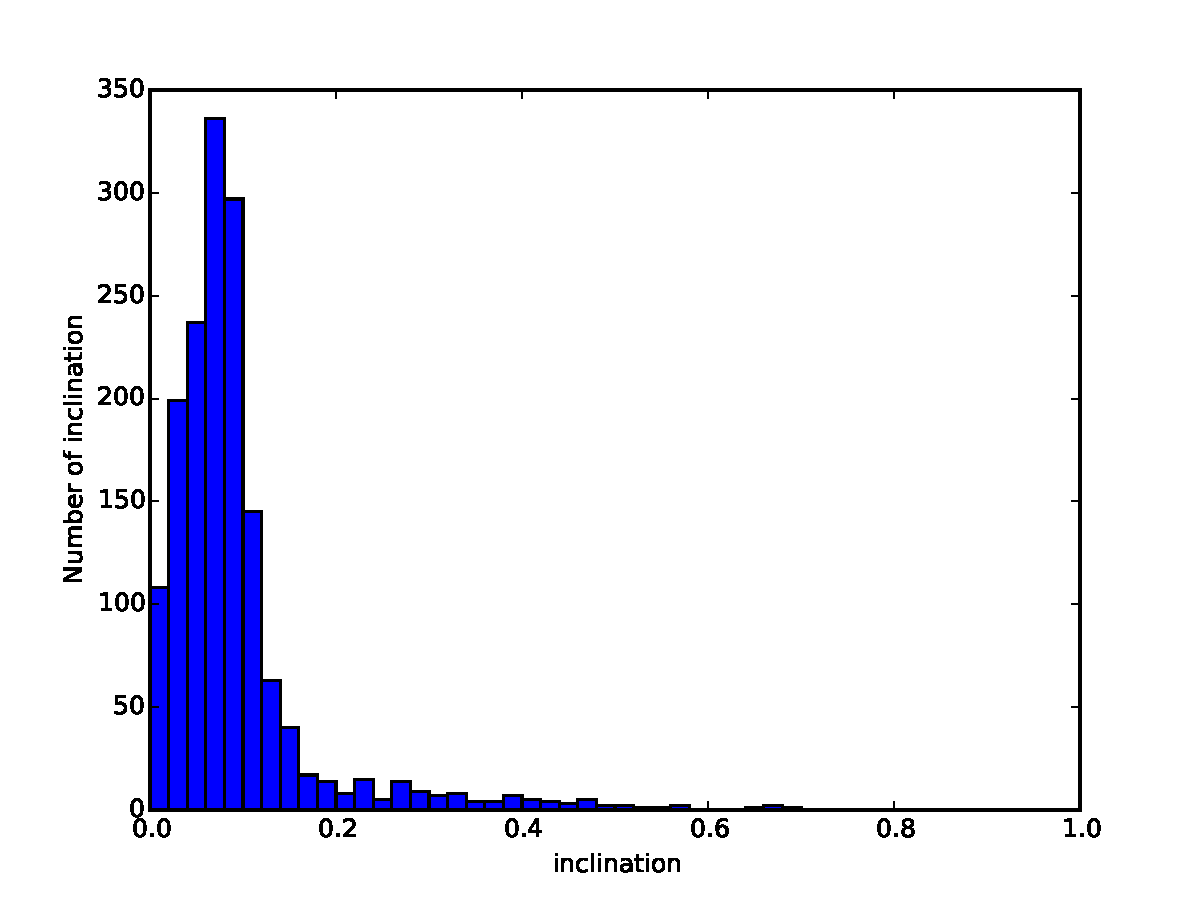
\includegraphics[width=0.8\hsize]{C:/master/mstudy/analysis/model/A_hist_all.pdf}
\caption{のこぎり波の傾きの分布}
\label{dist-inc}
\end{center}
\end{figure}
図 \ref{dist-inc} は 0.08 程度を山とするポアソン分布に見える.
 
また,自己相関は図 \ref{autoCorr-inc} となった.
ここではのこぎり波の幅によらず隣り合うのこぎり波のラグを 1 としている.
青色の範囲はのこぎり波の傾きにホワイトノイズが加わることを仮定した場合の信頼区間 95 \% の範囲であるが,用いたパッケージの影響で描写されたものでありここでは特に意味をなさない.
\begin{figure}[tb]
\begin{center}
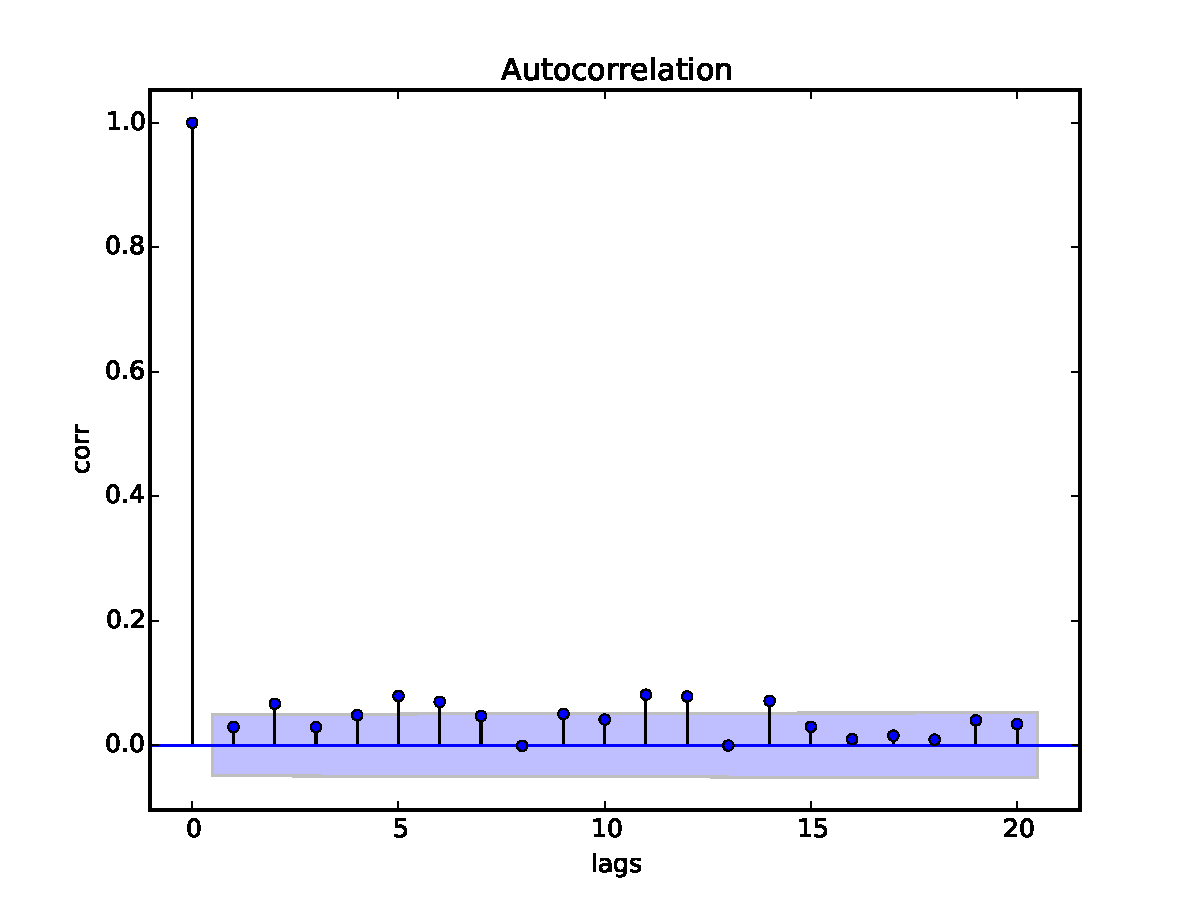
\includegraphics[width=0.8\hsize]{C:/master/mstudy/analysis/model/autoCorr-A.pdf}
\caption{のこぎり波の傾きの自己相関}
\label{autoCorr-inc}
\end{center}
\end{figure}
図 \ref{autoCorr-inc} より,あるのこぎり波とその直後 20 個ののこぎり波の傾きには相関は見られず,独立であると考えられる.

加えて,平均値と分散を表 \ref{stat-inc} に示す.
\begin{table}[tb]
\begin{center}
\caption{のこぎり波の傾きの統計量}
\label{stat-inc}
\begin{tabular}{|c|c|}
\hline
平均(少数第五位以下四捨五入)&分散(少数第五位以下四捨五入)\\
\hline
0.0915&0.0083\\
\hline
\end{tabular}
\end{center}
\end{table}
\subsection{のこぎり波の幅と傾きの相関}
のこぎり波の幅と傾きの相関は図 \ref{corr} で示したように,相関係数 -0.6 で緩やかな負の相関があるようだ.
幅が長い場合は傾きは小さくなっており,応答遅延の分布帯が極端に大きくならないようになっていると考えられる.
\begin{figure}[tb]
\begin{center}
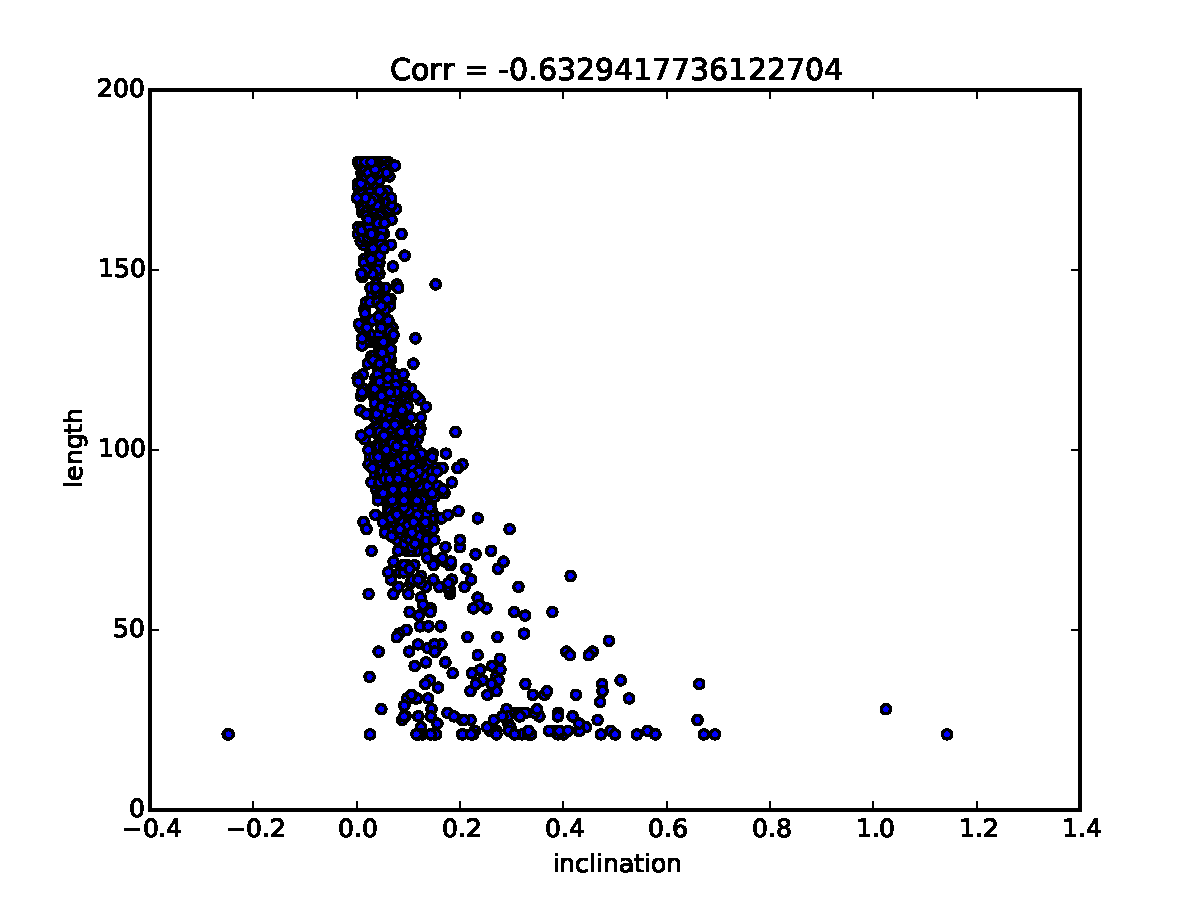
\includegraphics[width=0.8\hsize]{C:/master/mstudy/analysis/model/corr.pdf}
\caption{のこぎり波の幅と傾きの相関}
\label{corr}
\end{center}
\end{figure}

\section{格安SIMでの計測結果}
これまでの実験では曜日や時間帯に応じた顕著な傾向を見ることは困難であった.その要因の一つとして,これまで使用していた SIM の性能が悪くないため曜日や時間帯での差が見えずらくなっていることが考えられる.そこで,格安 SIM を用いて計測データを収集することで曜日や時間帯に応じた傾向を読み取れやすくなるのではないかと考えた.

8 月 20 日から 8 月 26 日までにかけて,格安 SIM を用いた場合とそうでない場合の比較実験を行った.
計測間隔は 15 秒である.
この計測結果を図 \ref{SIM1} と図 \ref{SIM2} に示す.
左側が格安 SIM を用いた場合の計測データである.
\begin{figure}[tb]
\begin{center}
\subfigure[8 月 20 日 (格安SIM)]{
\includegraphics[width=0.4\hsize]{C:/master/mstudy/analysis/FTP/lowSIM/plot-0820.pdf}
}~
\subfigure[8 月 20 日 (通常SIM)]{
\includegraphics[width=0.4\hsize]{C:/master/mstudy/analysis/FTP/lowSIMcomp/plot-0820.pdf}
}\\
\subfigure[8 月 21 日 (格安SIM)]{
\includegraphics[width=0.4\hsize]{C:/master/mstudy/analysis/FTP/lowSIM/plot-0821.pdf}
}~
\subfigure[8 月 21 日 (通常SIM)]{
\includegraphics[width=0.4\hsize]{C:/master/mstudy/analysis/FTP/lowSIMcomp/plot-0821.pdf}
}\\
\subfigure[8 月 22 日 (格安SIM)]{
\includegraphics[width=0.4\hsize]{C:/master/mstudy/analysis/FTP/lowSIM/plot-0822.pdf}
}~
\subfigure[8 月 22 日 (通常SIM)]{
\includegraphics[width=0.4\hsize]{C:/master/mstudy/analysis/FTP/lowSIMcomp/plot-0822.pdf}
}\\
\subfigure[8 月 23 日 (格安SIM)]{
\includegraphics[width=0.4\hsize]{C:/master/mstudy/analysis/FTP/lowSIM/plot-0823.pdf}
}~
\subfigure[8 月 23 日 (通常SIM)]{
\includegraphics[width=0.4\hsize]{C:/master/mstudy/analysis/FTP/lowSIMcomp/plot-0823.pdf}
}
\caption{格安SIMと通常SIMの比較}
\label{SIM1}
\end{center}
\end{figure}
\begin{figure}[tb]
\begin{center}
\subfigure[8 月 24 日 (格安SIM)]{
\includegraphics[width=0.4\hsize]{C:/master/mstudy/analysis/FTP/lowSIM/plot-0824.pdf}
}~
\subfigure[8 月 24 日 (通常SIM)]{
\includegraphics[width=0.4\hsize]{C:/master/mstudy/analysis/FTP/lowSIMcomp/plot-0824.pdf}
}\\
\subfigure[8 月 25 日 (格安SIM)]{
\includegraphics[width=0.4\hsize]{C:/master/mstudy/analysis/FTP/lowSIM/plot-0825.pdf}
}~
\subfigure[8 月 25 日 (通常SIM)]{
\includegraphics[width=0.4\hsize]{C:/master/mstudy/analysis/FTP/lowSIMcomp/plot-0825.pdf}
}\\
\subfigure[8 月 26 日 (格安SIM)]{
\includegraphics[width=0.4\hsize]{C:/master/mstudy/analysis/FTP/lowSIM/plot-0826.pdf}
}~
\subfigure[8 月 26 日 (通常SIM)]{
\includegraphics[width=0.4\hsize]{C:/master/mstudy/analysis/FTP/lowSIMcomp/plot-0826.pdf}
}
\caption{格安SIMと通常SIMの比較}
\label{SIM2}
\end{center}
\end{figure}

図より,格安 SIM を用いた場合とそうでない場合の間に目に見えた差はないように思える.
また,具体的な統計量は表 \ref{sim} に示した.
また,8 月 22 日の 16 時以降から,格安 SIM の場合とそうでない場合両方で応答遅延の下振れが激しくなっていた.具体的な理由までは分からないが,SIM に関わらず同時期に発生していることから,二台の raspberry pi から AWS サーバ までの通信路で共通する箇所で発生した何らかの原因によるものだと考えられる.
\begin{table}[tb]
\begin{center}
\caption{格安SIMと通常SIMの平均と分散の比較}
\label{sim}
\begin{tabular}{|c|c|c|c|c|}
\hline
&\multicolumn{2}{|c|}{平均} &\multicolumn{2}{|c|}{分散}\\
&格安SIM&通常SIM&格安SIM&通常SIM\\
\hline
8 月 20 日&77&77&61&46\\
\hline
8 月 21 日&79&80&93&61\\
\hline
8 月 22 日&80&78&149&69\\
\hline
8 月 23 日&75&75&231&137\\
\hline
8 月 24 日&77&73&272&223\\
\hline
8 月 25 日&75&75&139&302\\
\hline
8 月 26 日&75&77&135&233\\
\hline
\end{tabular}
\end{center}
\end{table}
\section{FTPを併用した計測結果}
10 回の ping 応答遅延計測を 10 ミリ秒間隔で行い,これを 15 秒毎に繰り返す実験では,10 ミリ秒間隔で行う 10 回の計測の一回目が大きく二つ目以降から小さくなっていく傾向が見て取れた.
これは,二回目以降の計測では一回目の計測の影響で eNodeB でのリソース割り当てが高速化しているからではないかと考えられる.そこでここでは,この高速化を引き起こす原因が ICMP のプロトコルに依存するものなのかどうかを調べるため,FTP による通信をバックグラウンドで行いながらの以下の二つの実験を行う.

\subsection{15秒間隔での計測}
FTP 通信下においても 15 秒間隔での ping 計測値が 70 ミリ秒から 90 ミリ秒までの間に多く分布するのかどうかを調べる.もし 10 ミリ秒間隔での計測値のように 30 ミリ秒から 50 ミリ秒の間に多く分布するのであれば,他の通信が行われている状況での応答遅延の分布帯は小さなものになると考えられる.

FTP 通信を併用した 15 秒間隔での計測を行った.
具体的な計測手順をいかに示す.
\begin{enumerate}
\item 計測開始時に一台の Raspberry Pi から AWS サーバに FTP 接続を行う.
\item 2 M バイト(約 2 秒) の送信を開始する.
\item 2. の開始の 0.5 秒後に ping 計測を行う.同時に各 ping コマンドの実行直前の時刻も取得する.
\item 15 秒後に 2. に戻る.終了条件は 1. から 1 時間経過した場合とする.
\end{enumerate}
また,比較対象として直前と別日の同一曜日の同一時間帯に FTP 通信を用いない場合の計測も行った.
直後に関しては何らかのミスにより計測に失敗しておりました.
結果を図 \ref{15s} に示す.
また,平均と分散を表 \ref{15s-stat} に示す.
\begin{figure}[tb]
\begin{center}
\subfigure[直前]{
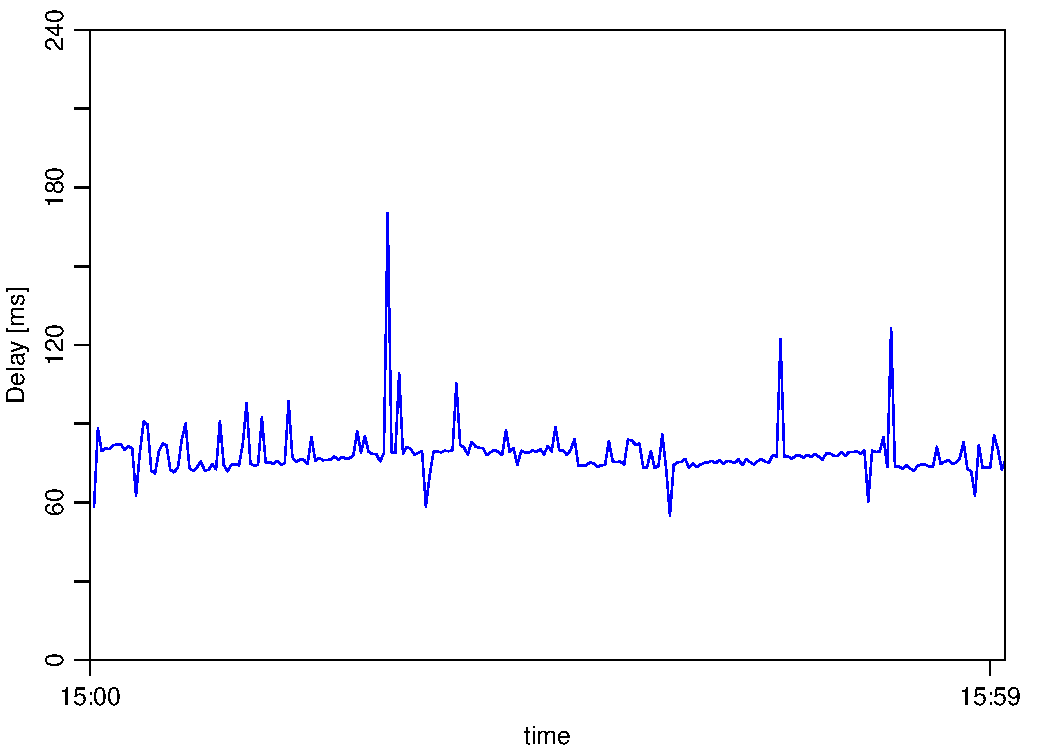
\includegraphics[width=0.5\hsize]{C:/master/mstudy/analysis/FTP/15sFTP/exam2-before.pdf}
}~
\subfigure[本実験]{
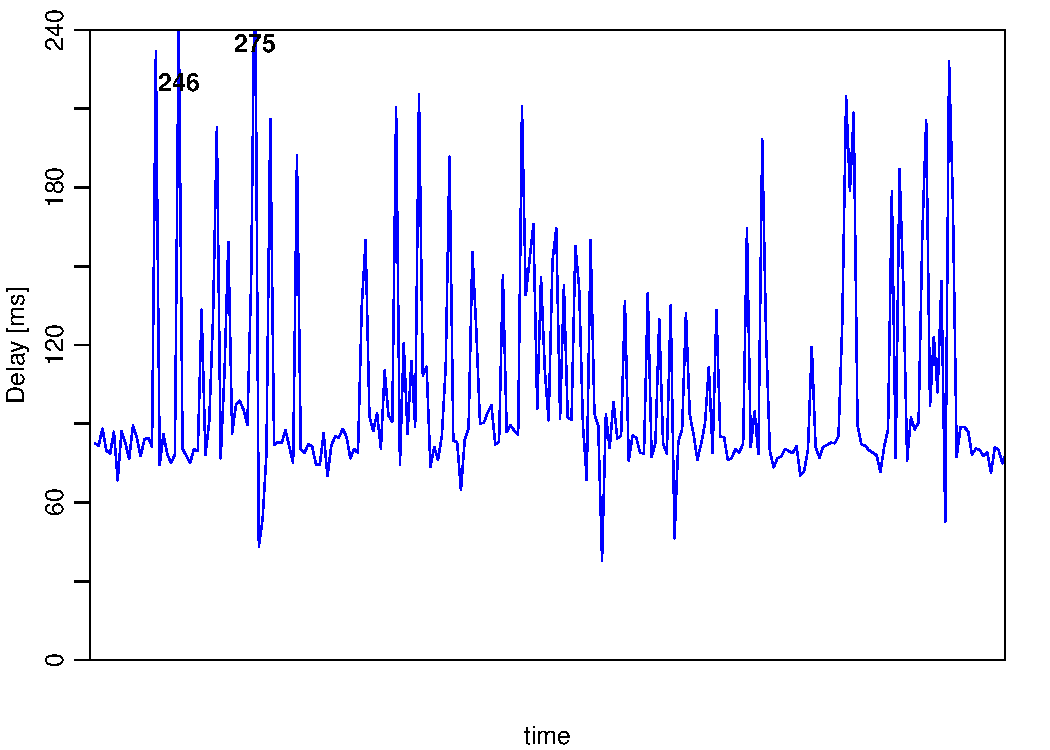
\includegraphics[width=0.5\hsize]{C:/master/mstudy/analysis/FTP/15sFTP/exam2.pdf}
}\\
\subfigure[別日]{
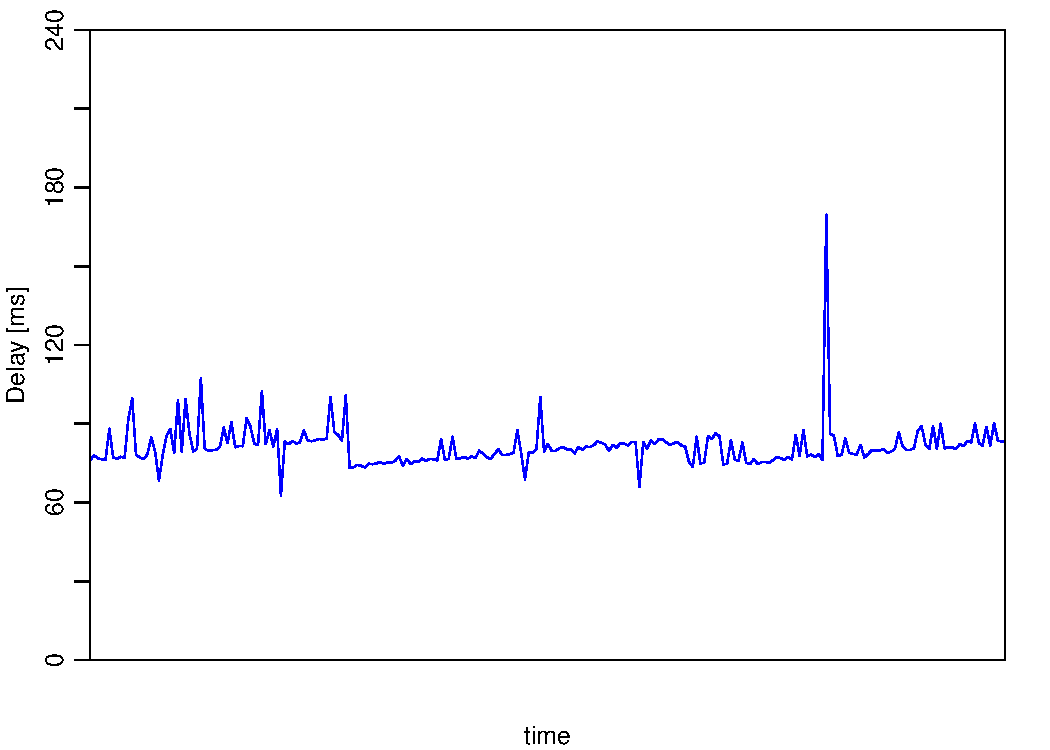
\includegraphics[width=0.5\hsize]{C:/master/mstudy/analysis/FTP/15sFTP/exam2-other.pdf}
}
\caption{FTP を併用した 15 秒間隔の実験}
\label{15s}
\end{center}
\end{figure}
\begin{table}[tb]
\begin{center}
\caption{FTP を併用した 15 秒間隔の実験の平均と分散}
\label{15s-stat}
\begin{tabular}{|c|c|c|}
\hline
&平均 &分散\\
\hline
直前&78&88\\
\hline
本実験&102&1574\\
\hline
別日&81&66\\
\hline
\end{tabular}
\end{center}
\end{table}
図より,FTP を併用しても分布帯は小さくならないようだ.このことから,他の通信の最中であればリソース割り当ての高速化により応答遅延が小さくなるのではないかという仮説は正しくないようだ.
また,大きな応答遅延の発生頻度が極端に高くなっていた.
これは,FTP 通信に raspberry pi 上の計算資源もしくは eNB の無線リソースが割かれ ICMP の ping の処理が後回しにされているのではないかと考えられる.

\subsection{10ミリ秒間隔での計測}
FTP 通信下においても 10 ミリ秒間隔の計測が減少傾向を示すのかを調べる.もし一回目の計測から小さな値を取るのであれば,ICMP に限らず他に通信が行われている状況での ping 応答遅延は小さくなると考えられる.

FTP 通信を併用した 10 ミリ秒間隔での計測を行った.
具体的な計測手順を以下に示す.
\begin{enumerate}
\item 計測開始時に一台の Raspberry Pi から AWS サーバに FTP 接続を行う.
\item 2 M バイト(約 2 秒間) の送信を開始する.
\item 2. の開始の 0.5 秒後から 10 ミリ行間隔で 10 回の ping 計測を行う.同時に各 ping コマンドの実行直前の時刻も取得する.
\item 15 秒後に 2. に戻る.終了条件は 1. から 20 分経過した場合とする.
\end{enumerate}
また,比較対象として直前と別日の同一曜日の同一時間帯に FTP 通信を用いない場合の計測も行った.
本計測は 8 月 27 日と 28 日の二日行った.
結果を図 \ref{10ms} から図 \ref{10ms-2} に示す.
\begin{figure}[tb]
\begin{center}
\subfigure[直前,インデックス 1 から 200 まで]{
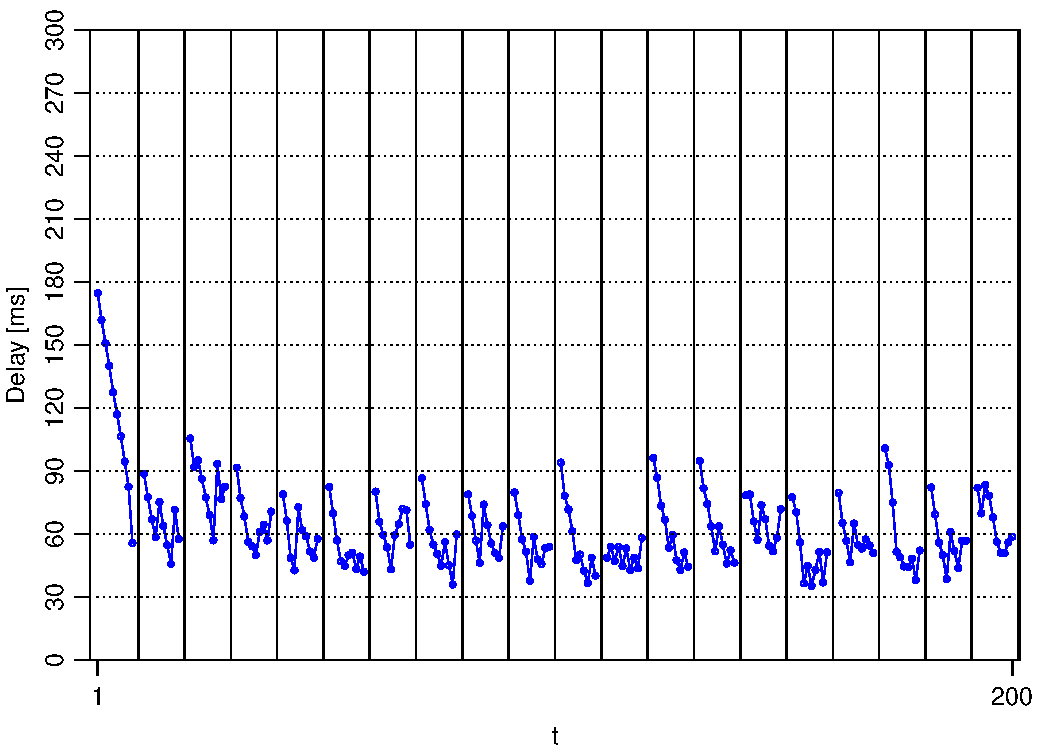
\includegraphics[width=0.4\hsize]{C:/master/mstudy/analysis/FTP/10msFTP/day1/exam1-day1-before-1st.pdf}
}~
\subfigure[直前,インデックス 201 から 400 まで]{
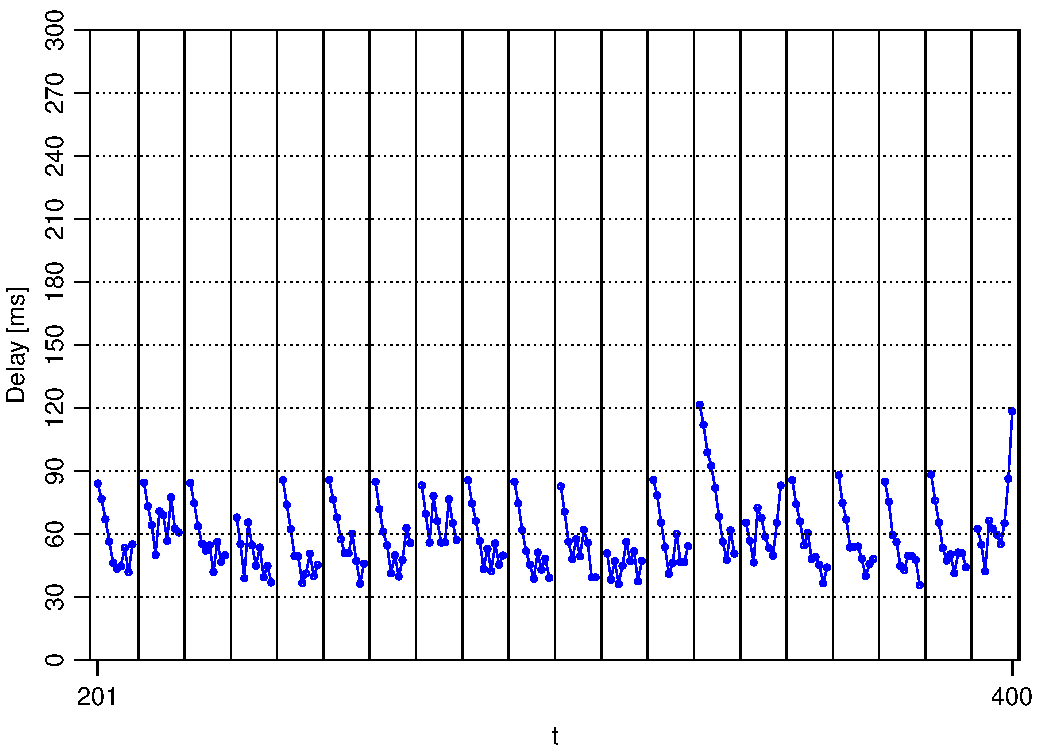
\includegraphics[width=0.4\hsize]{C:/master/mstudy/analysis/FTP/10msFTP/day1/exam1-day1-before-2nd.pdf}
}\\
\subfigure[直前,インデックス 401 から 600 まで]{
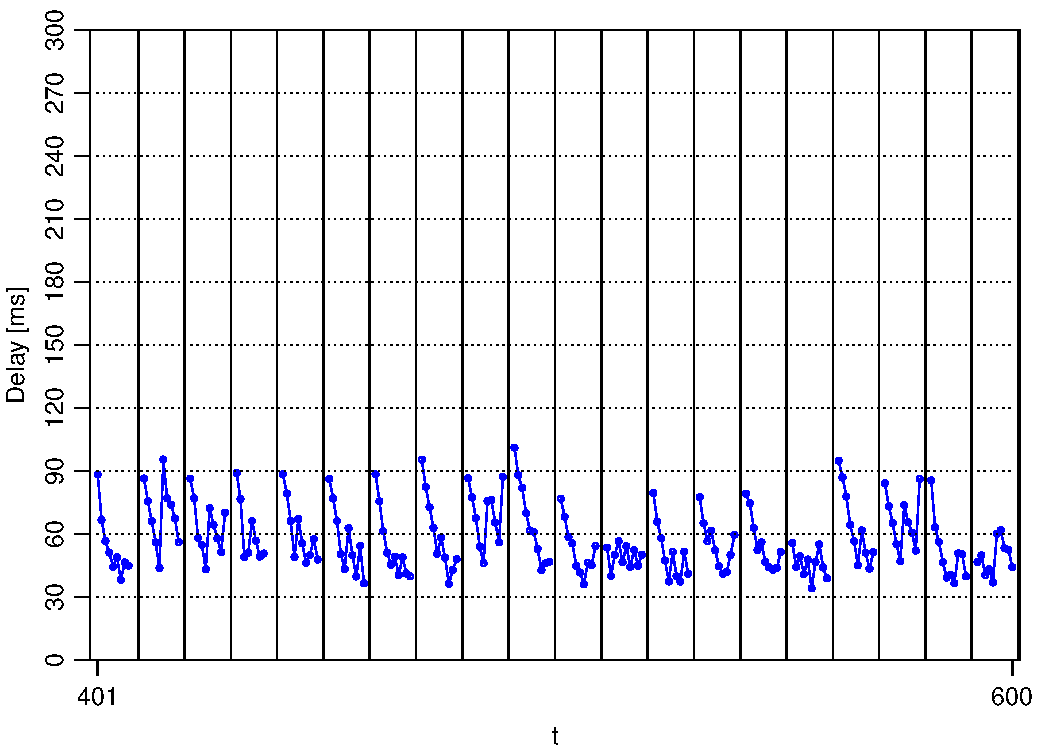
\includegraphics[width=0.4\hsize]{C:/master/mstudy/analysis/FTP/10msFTP/day1/exam1-day1-before-3rd.pdf}
}~
\subfigure[直前,インデックス 601 から 800 まで]{
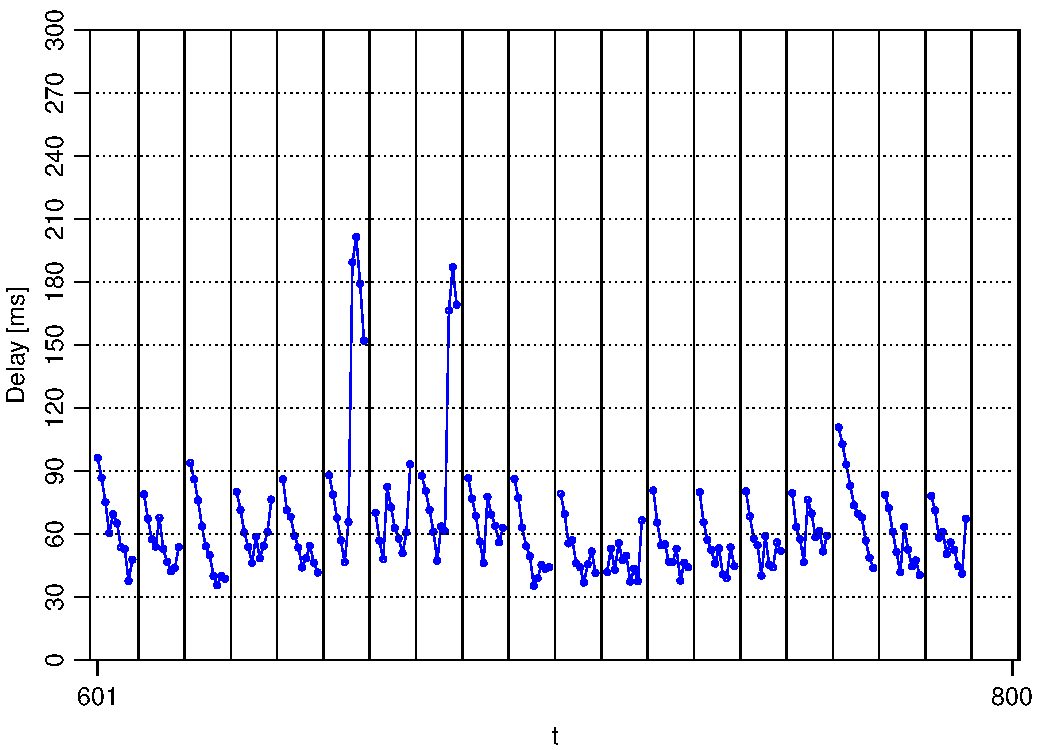
\includegraphics[width=0.4\hsize]{C:/master/mstudy/analysis/FTP/10msFTP/day1/exam1-day1-before-4th.pdf}
}\\
\subfigure[本実験,インデックス 1 から 200 まで]{
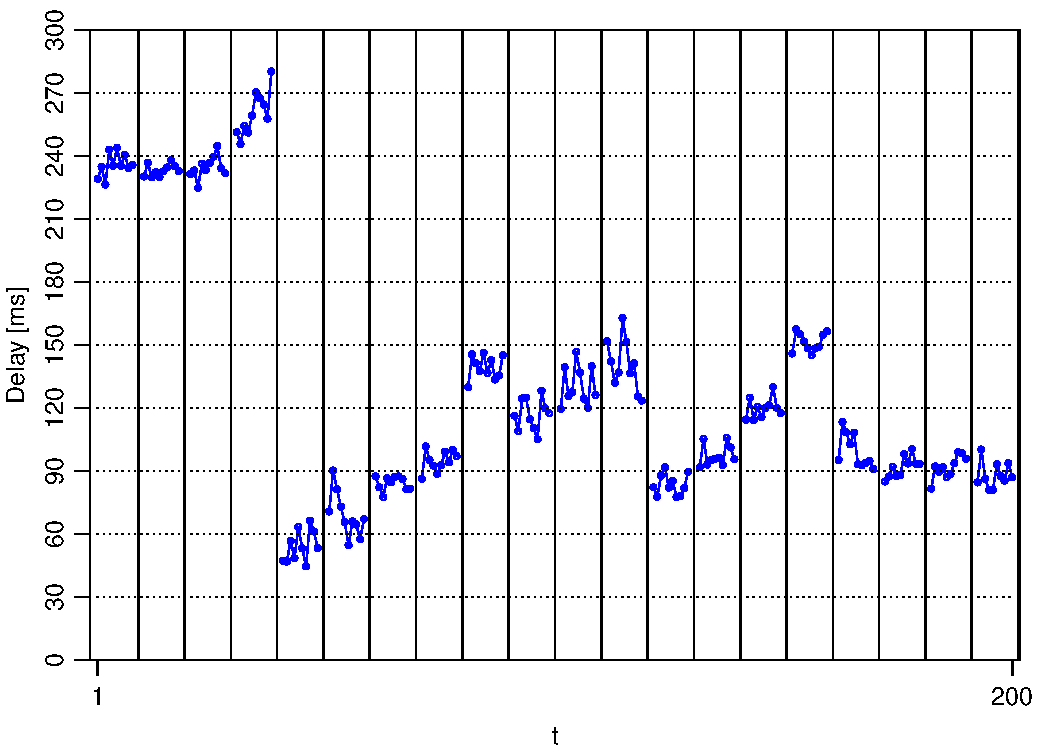
\includegraphics[width=0.4\hsize]{C:/master/mstudy/analysis/FTP/10msFTP/day1/exam1-day1-1st.pdf}
}~
\subfigure[本実験,インデックス 201 から 400 まで]{
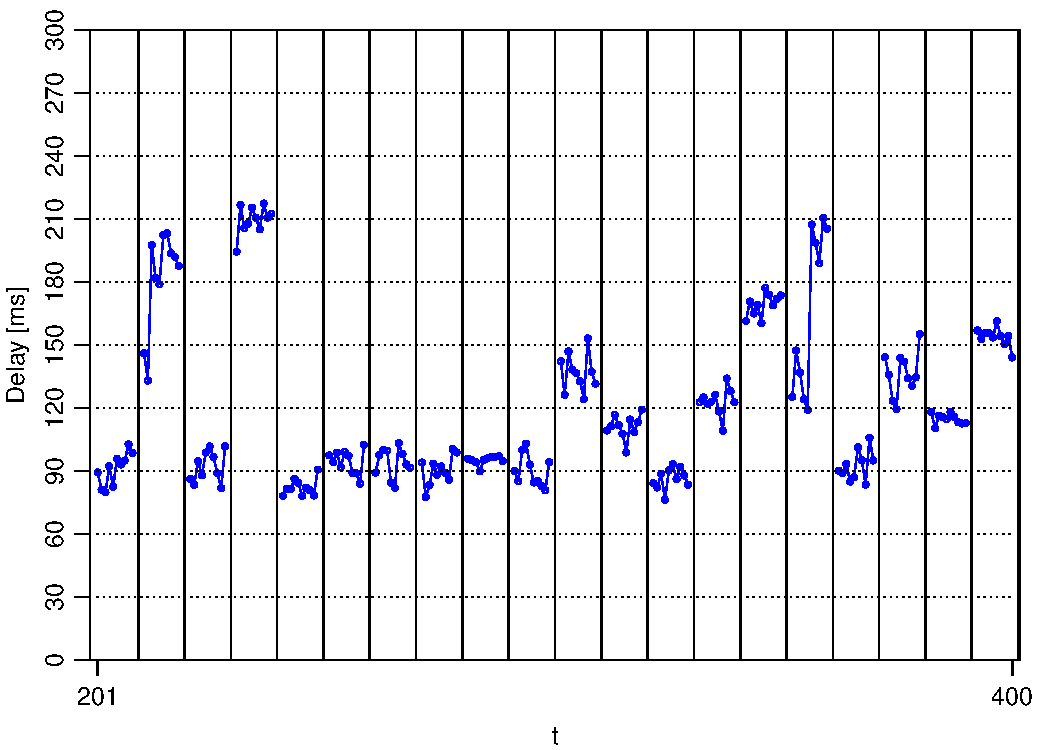
\includegraphics[width=0.4\hsize]{C:/master/mstudy/analysis/FTP/10msFTP/day1/exam1-day1-2nd.pdf}
}\\
\subfigure[本実験,インデックス 401 から 600 まで]{
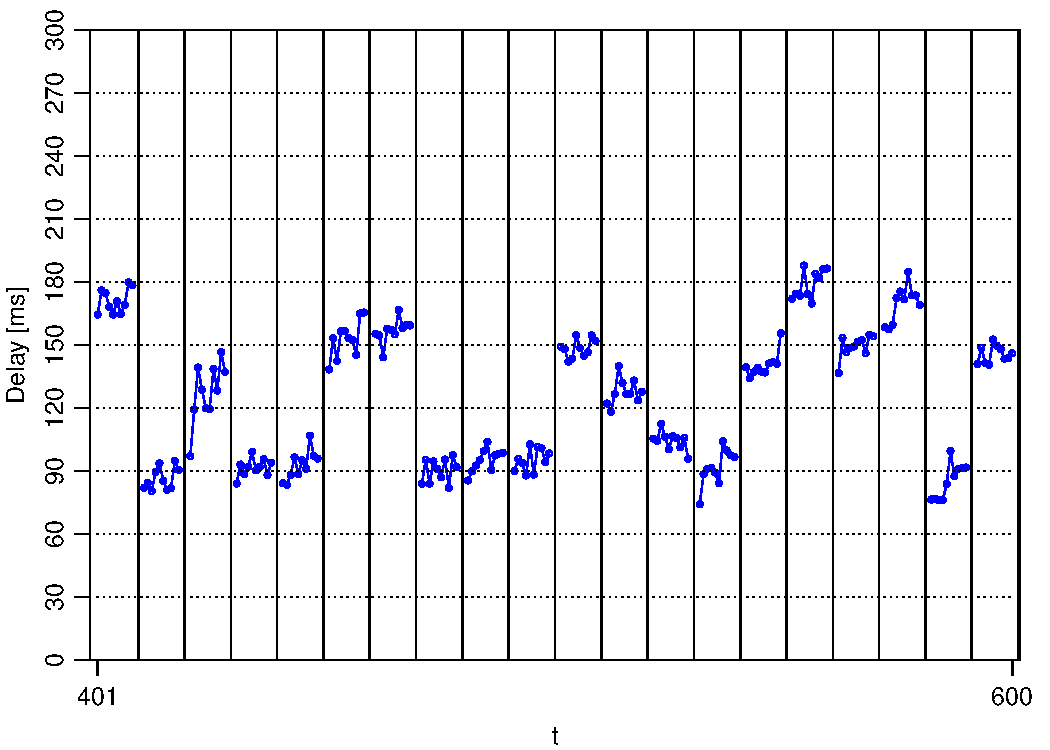
\includegraphics[width=0.4\hsize]{C:/master/mstudy/analysis/FTP/10msFTP/day1/exam1-day1-3rd.pdf}
}~
\subfigure[本実験,インデックス 601 から 800 まで]{
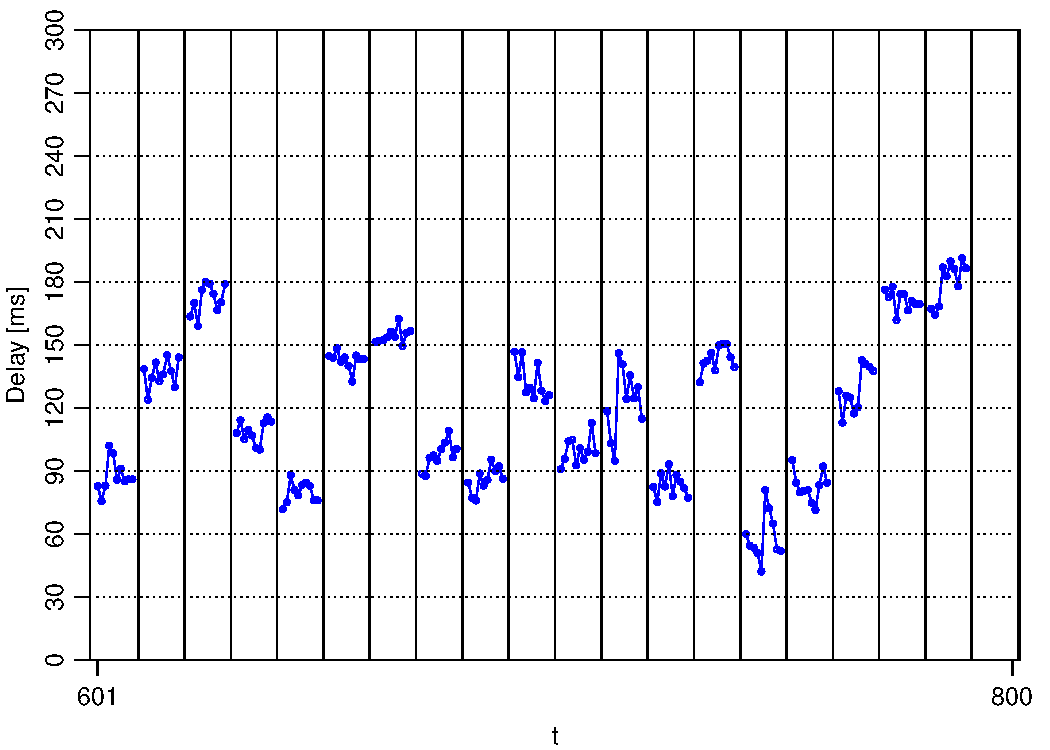
\includegraphics[width=0.4\hsize]{C:/master/mstudy/analysis/FTP/10msFTP/day1/exam1-day1-4th.pdf}
}
\caption{FTP を併用した 10 ミリ秒間隔の実験(一回目)}
\label{10ms}
\end{center}
\end{figure}
\begin{figure}[tb]
\begin{center}
\subfigure[直後,インデックス 1 から 200 まで]{
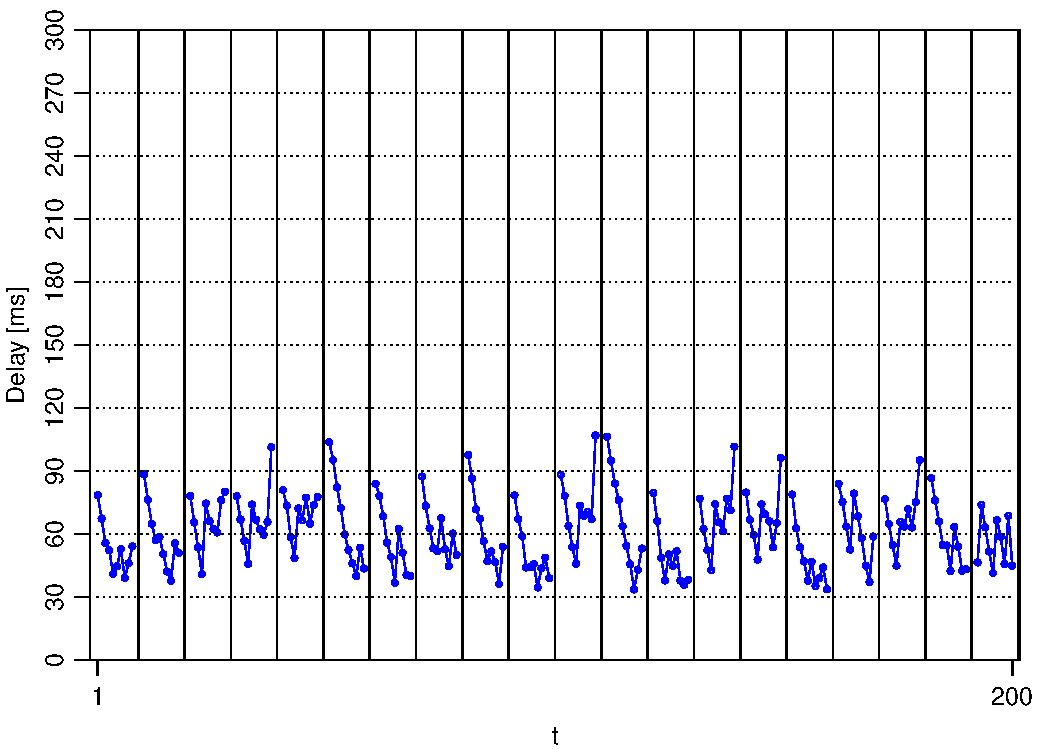
\includegraphics[width=0.4\hsize]{C:/master/mstudy/analysis/FTP/10msFTP/day1/exam1-day1-after-1st.pdf}
}~
\subfigure[直後,インデックス 201 から 400 まで]{
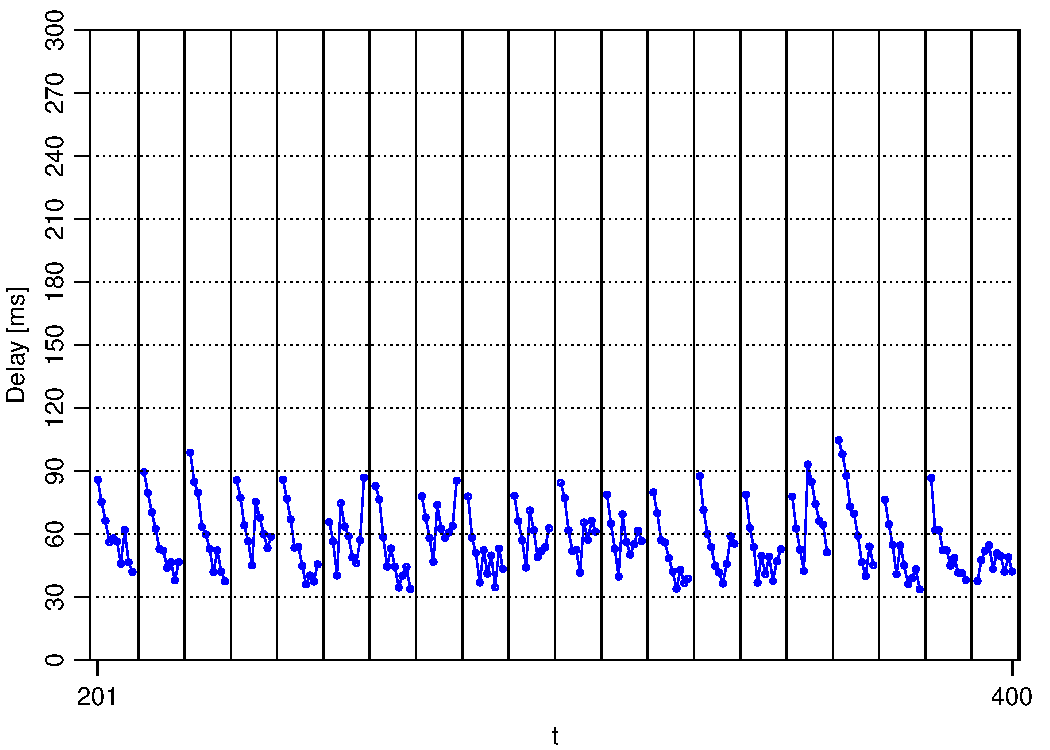
\includegraphics[width=0.4\hsize]{C:/master/mstudy/analysis/FTP/10msFTP/day1/exam1-day1-after-2nd.pdf}
}\\
\subfigure[直後,インデックス 401 から 600 まで]{
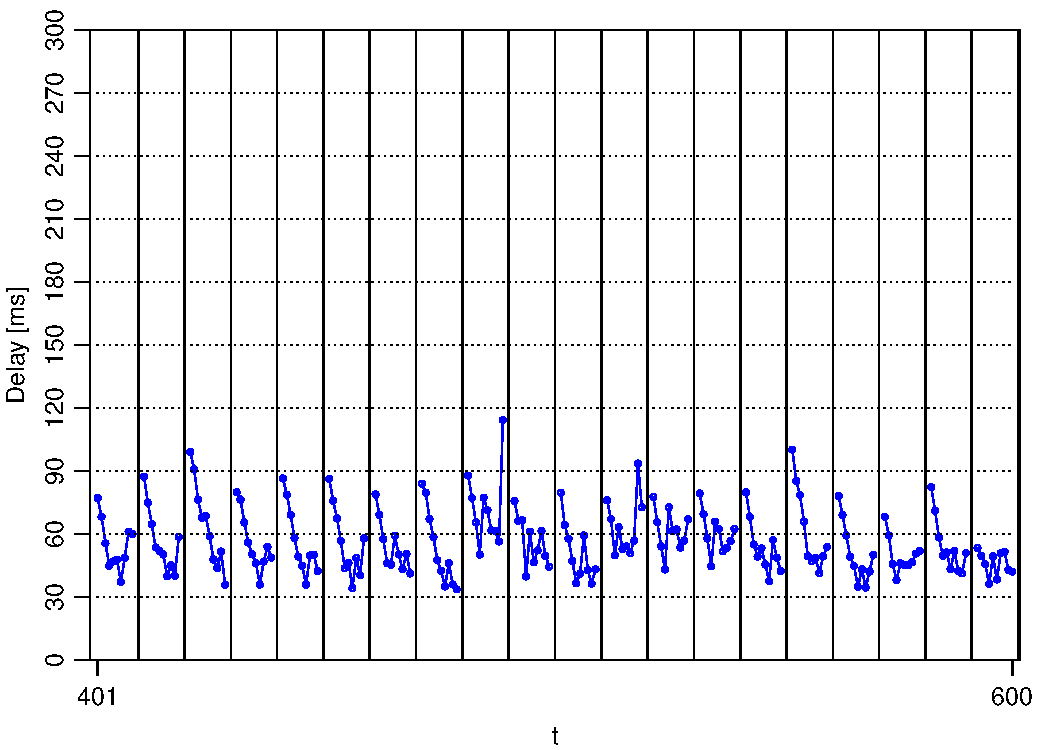
\includegraphics[width=0.4\hsize]{C:/master/mstudy/analysis/FTP/10msFTP/day1/exam1-day1-after-3rd.pdf}
}~
\subfigure[直後,インデックス 601 から 800 まで]{
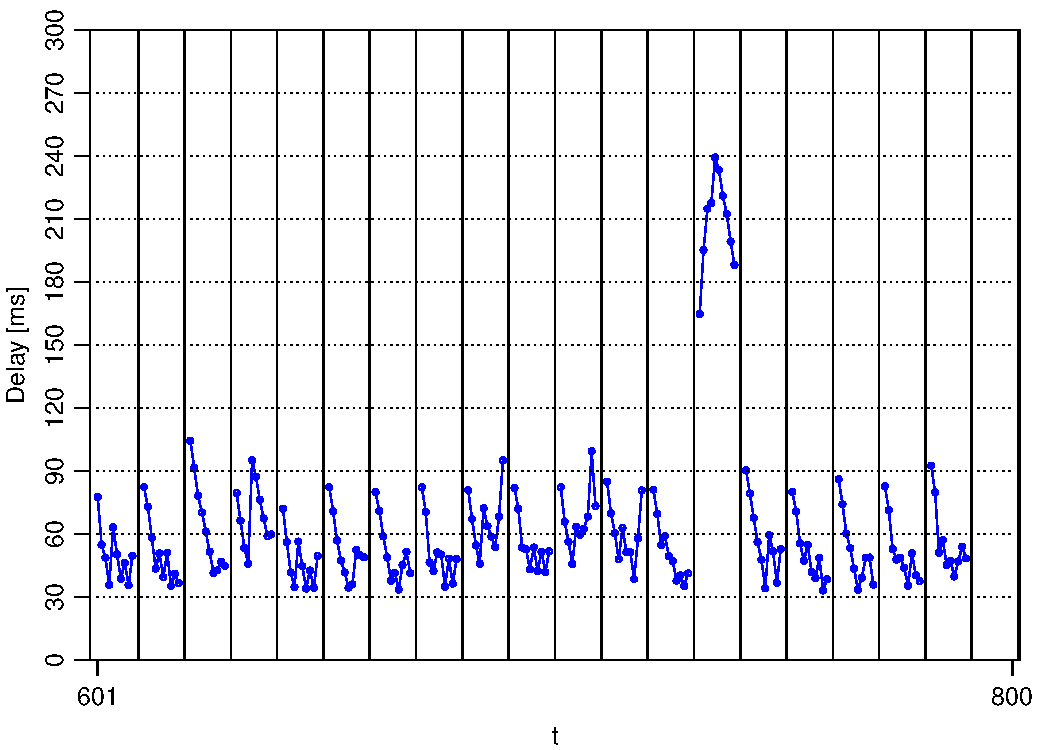
\includegraphics[width=0.4\hsize]{C:/master/mstudy/analysis/FTP/10msFTP/day1/exam1-day1-after-4th.pdf}
}\\
\subfigure[別日,インデックス 1 から 200 まで]{
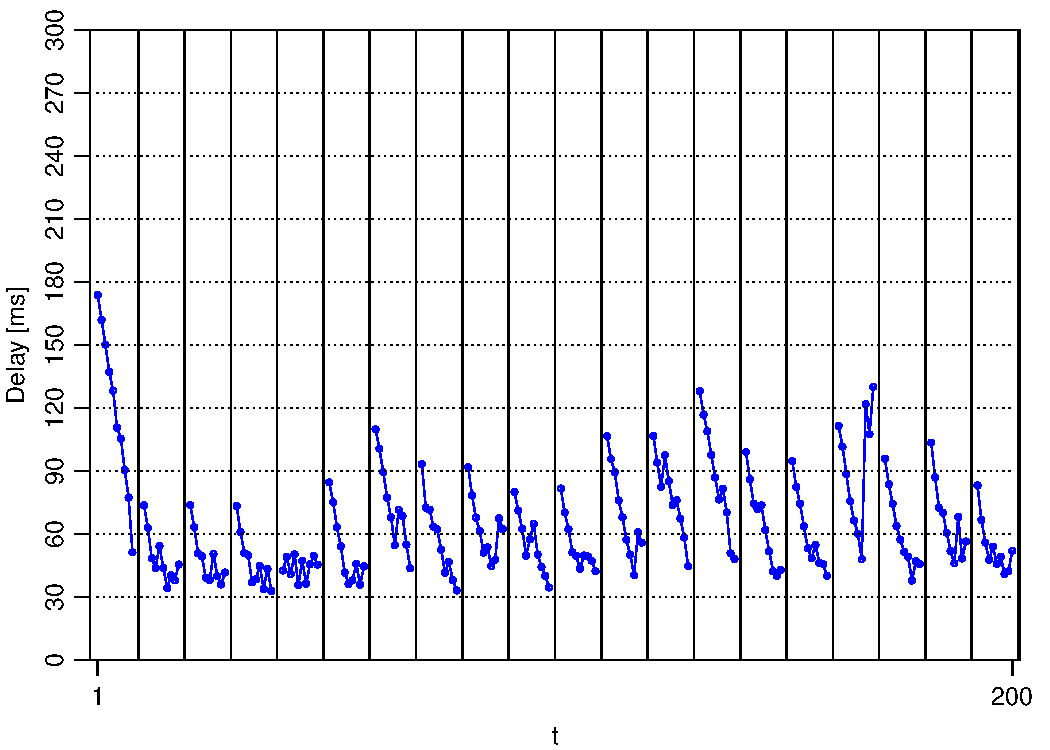
\includegraphics[width=0.4\hsize]{C:/master/mstudy/analysis/FTP/10msFTP/day1/exam1-day1-other-1st.pdf}
}~
\subfigure[別日,インデックス 201 から 400 まで]{
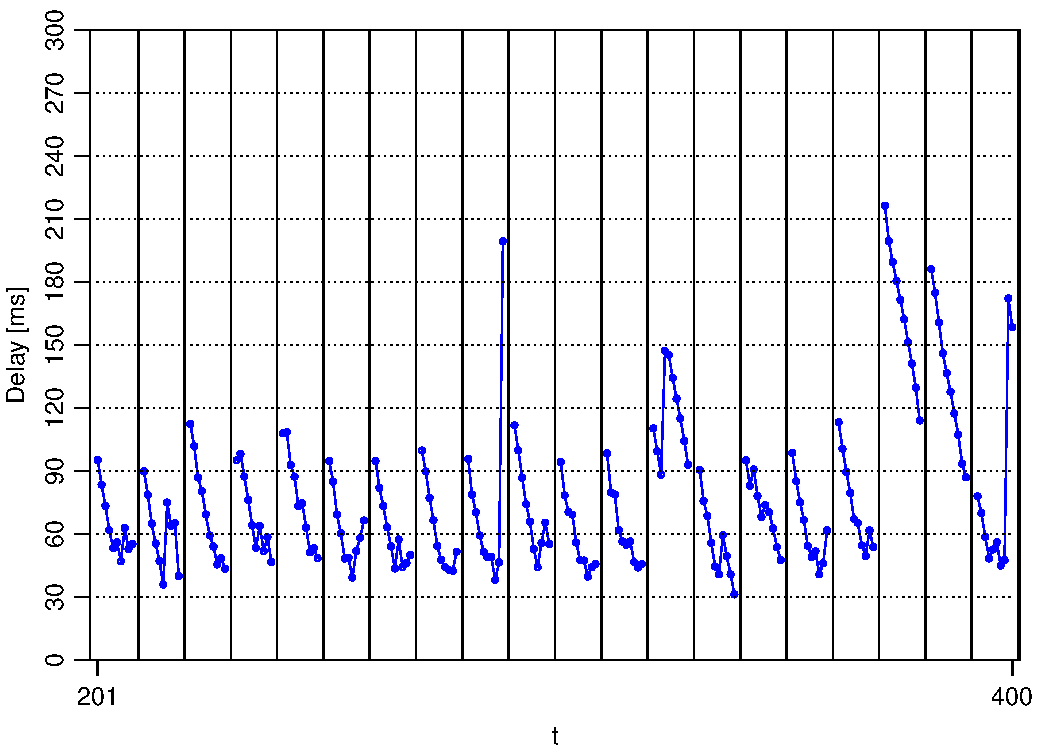
\includegraphics[width=0.4\hsize]{C:/master/mstudy/analysis/FTP/10msFTP/day1/exam1-day1-other-2nd.pdf}
}\\
\subfigure[別日,インデックス 401 から 600 まで]{
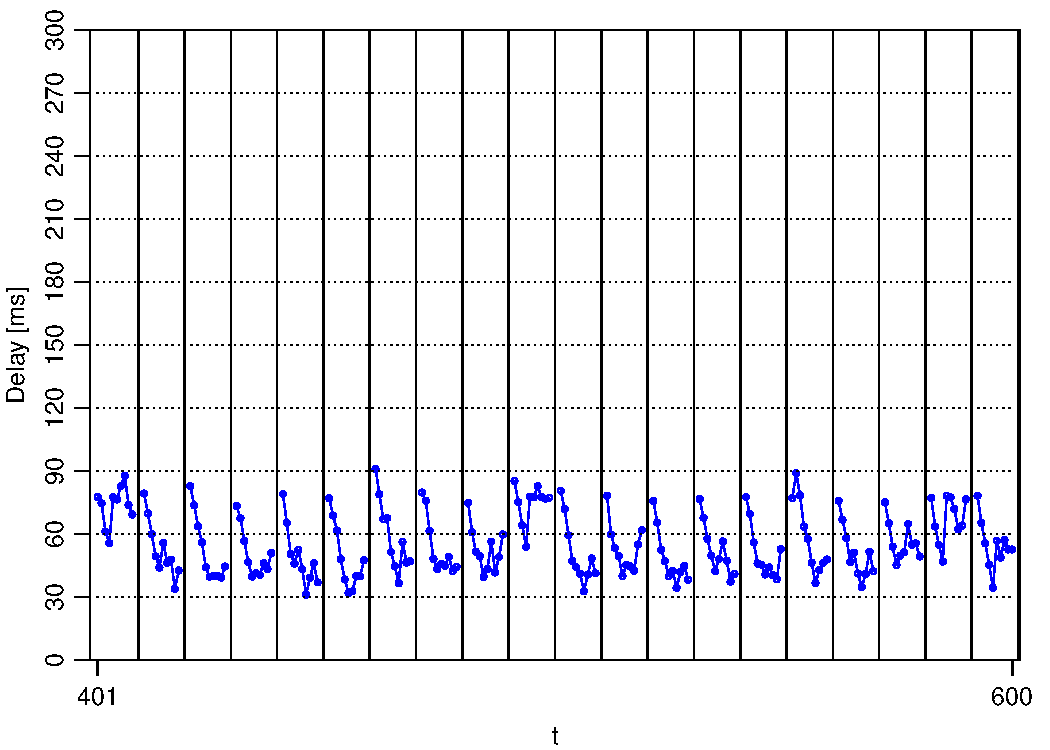
\includegraphics[width=0.4\hsize]{C:/master/mstudy/analysis/FTP/10msFTP/day1/exam1-day1-other-3rd.pdf}
}~
\subfigure[別日,インデックス 601 から 800 まで]{
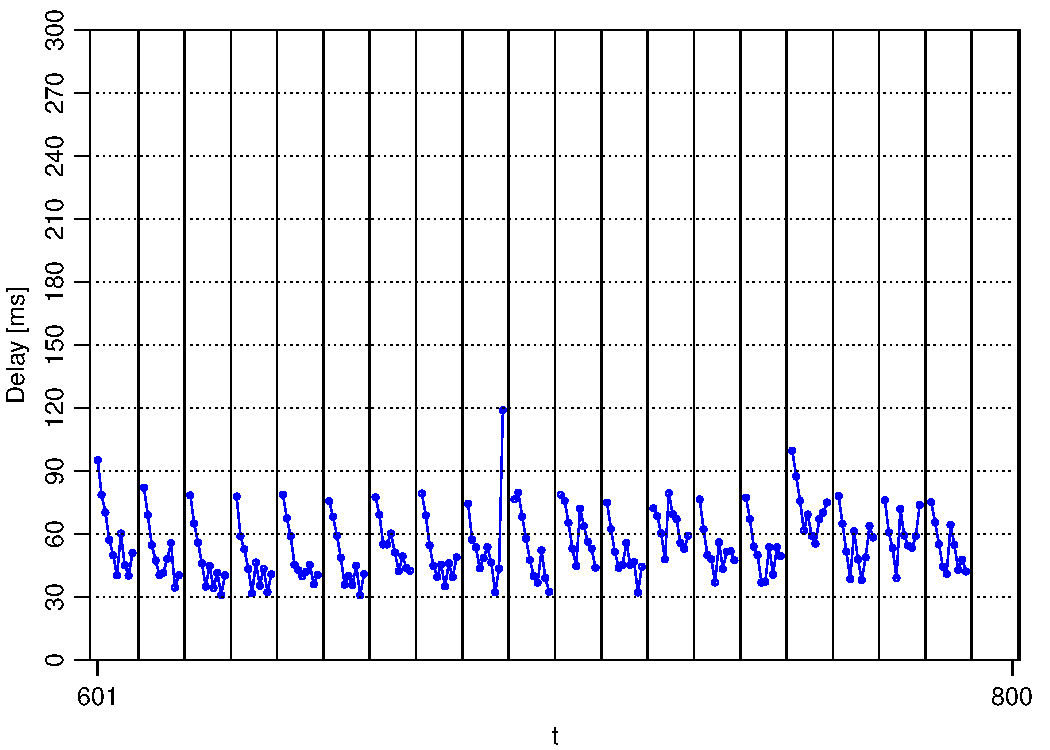
\includegraphics[width=0.4\hsize]{C:/master/mstudy/analysis/FTP/10msFTP/day1/exam1-day1-other-4th.pdf}
}
\caption{FTP を併用した 10 ミリ秒間隔の実験(一回目)}
\end{center}
\end{figure}

\begin{figure}[tb]
\begin{center}
\subfigure[直前,インデックス 1 から 200 まで]{
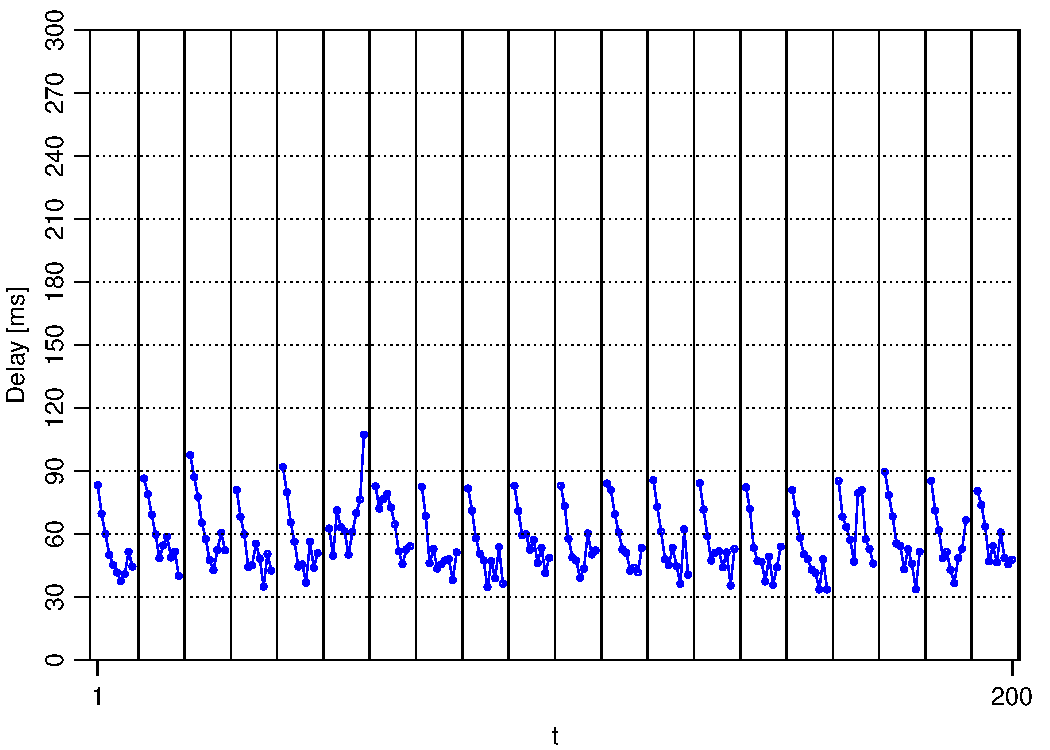
\includegraphics[width=0.4\hsize]{C:/master/mstudy/analysis/FTP/10msFTP/day2/exam1-day2-before-1st.pdf}
}~
\subfigure[直前,インデックス 201 から 400 まで]{
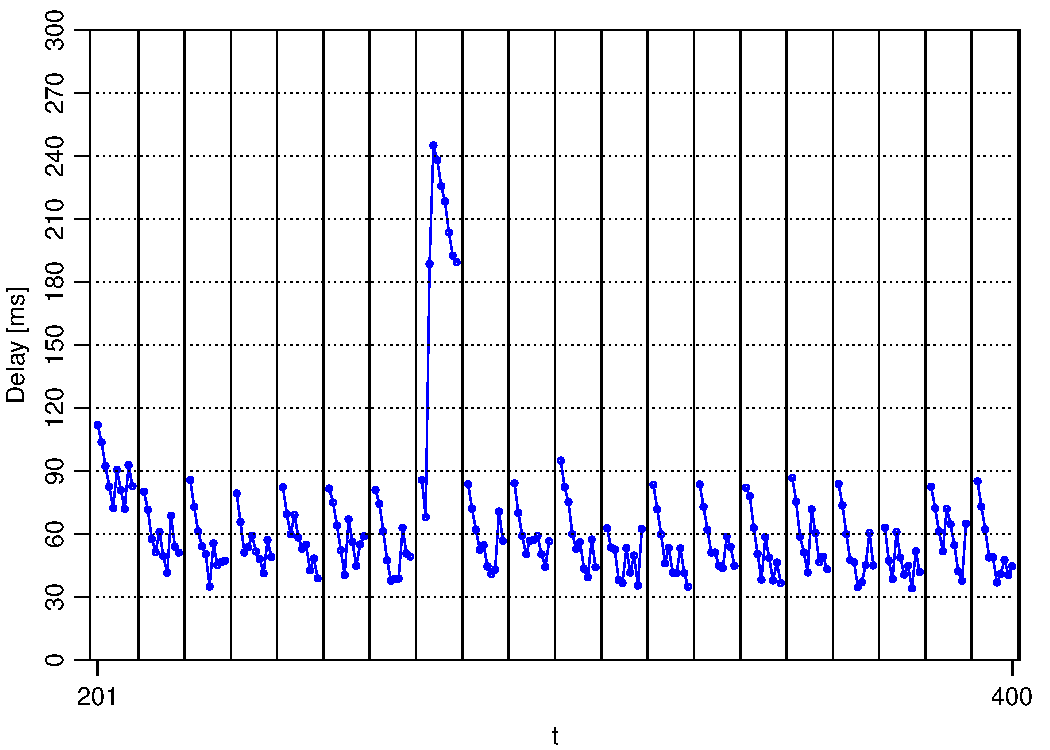
\includegraphics[width=0.4\hsize]{C:/master/mstudy/analysis/FTP/10msFTP/day2/exam1-day2-before-2nd.pdf}
}\\
\subfigure[直前,インデックス 401 から 600 まで]{
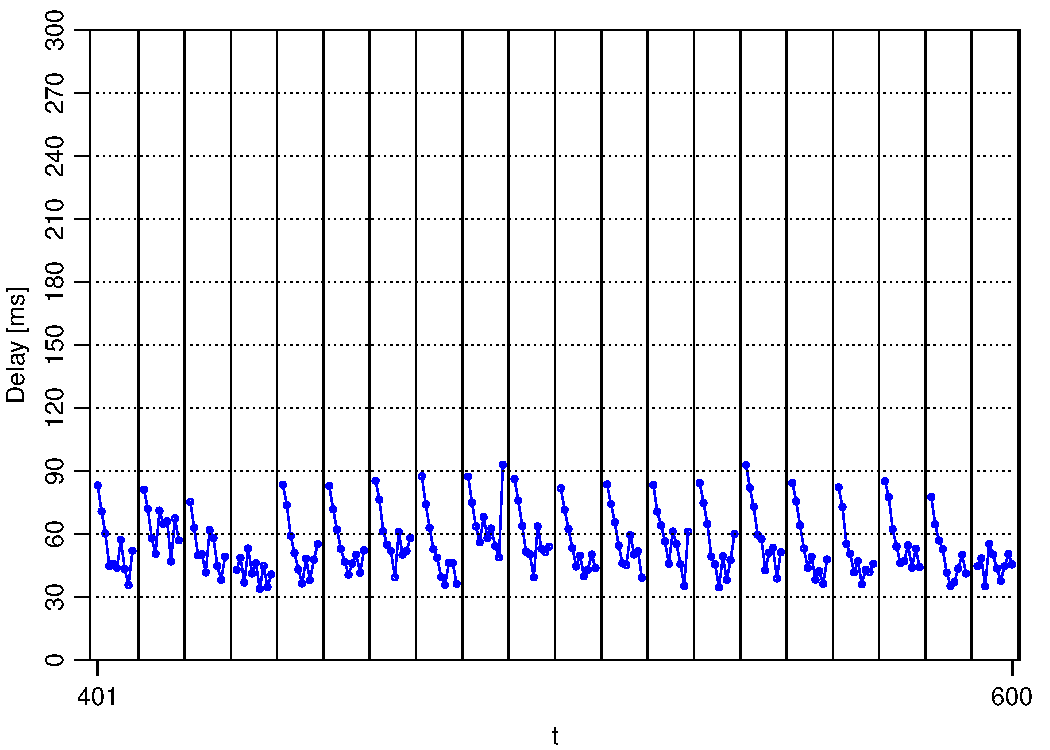
\includegraphics[width=0.4\hsize]{C:/master/mstudy/analysis/FTP/10msFTP/day2/exam1-day2-before-3rd.pdf}
}~
\subfigure[直前,インデックス 601 から 800 まで]{
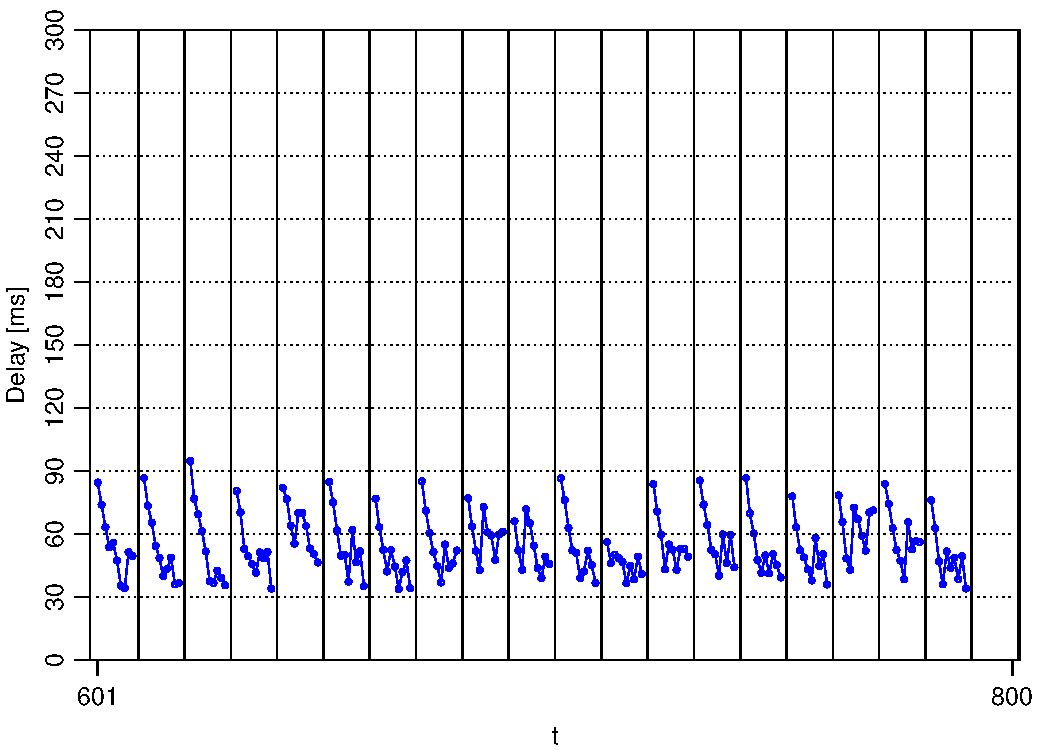
\includegraphics[width=0.4\hsize]{C:/master/mstudy/analysis/FTP/10msFTP/day2/exam1-day2-before-4th.pdf}
}\\
\subfigure[本実験,インデックス 1 から 200 まで]{
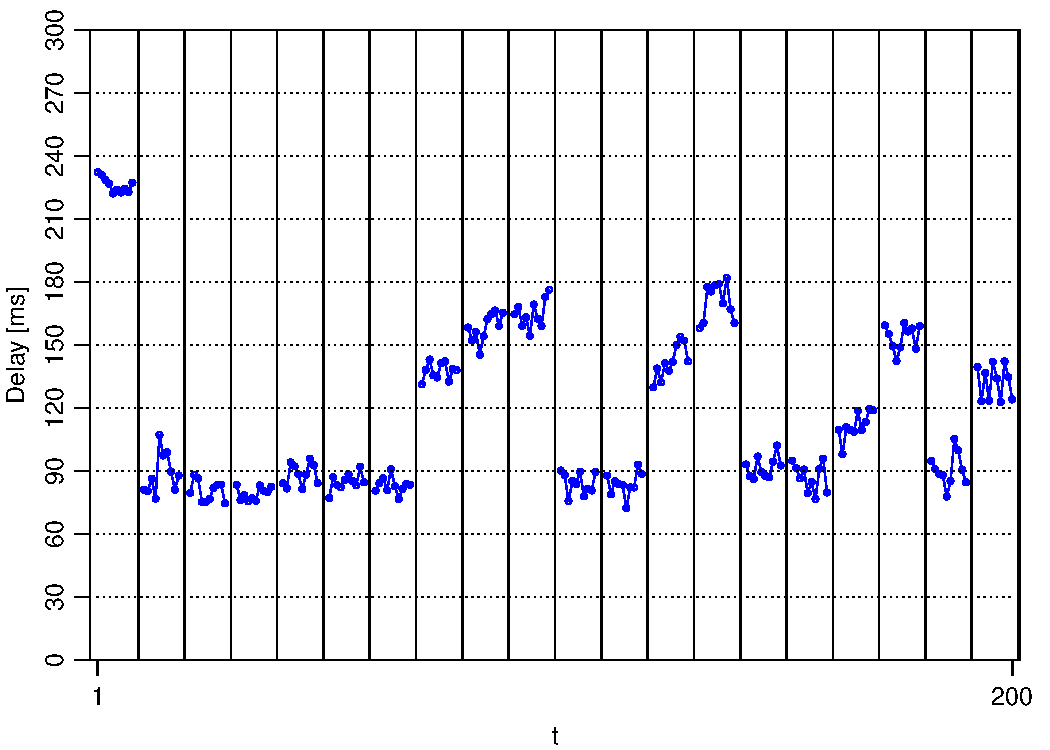
\includegraphics[width=0.4\hsize]{C:/master/mstudy/analysis/FTP/10msFTP/day2/exam1-day2-1st.pdf}
}~
\subfigure[本実験,インデックス 201 から 400 まで]{
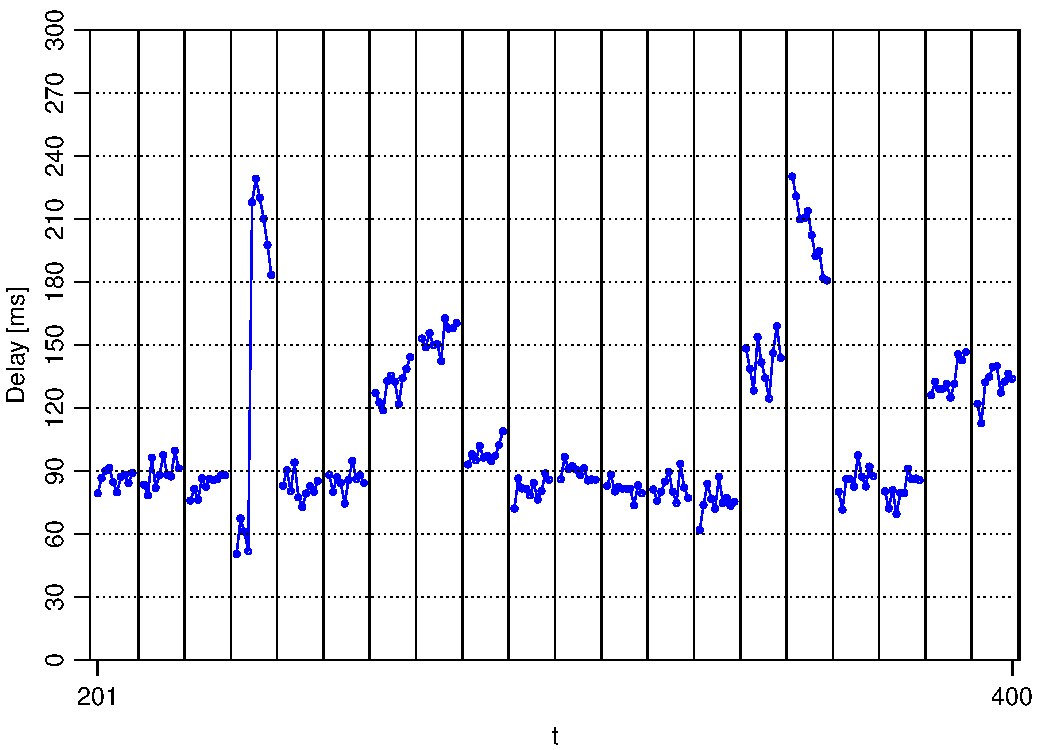
\includegraphics[width=0.4\hsize]{C:/master/mstudy/analysis/FTP/10msFTP/day2/exam1-day2-2nd.pdf}
}\\
\subfigure[本実験,インデックス 401 から 600 まで]{
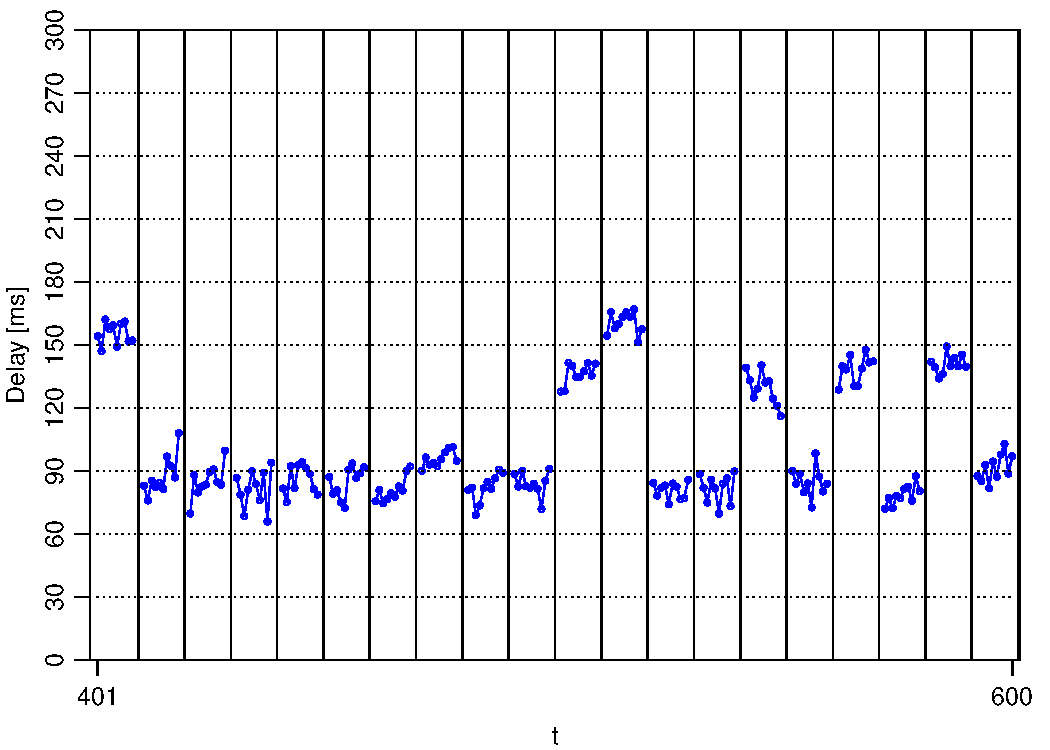
\includegraphics[width=0.4\hsize]{C:/master/mstudy/analysis/FTP/10msFTP/day2/exam1-day2-3rd.pdf}
}~
\subfigure[本実験,インデックス 601 から 800 まで]{
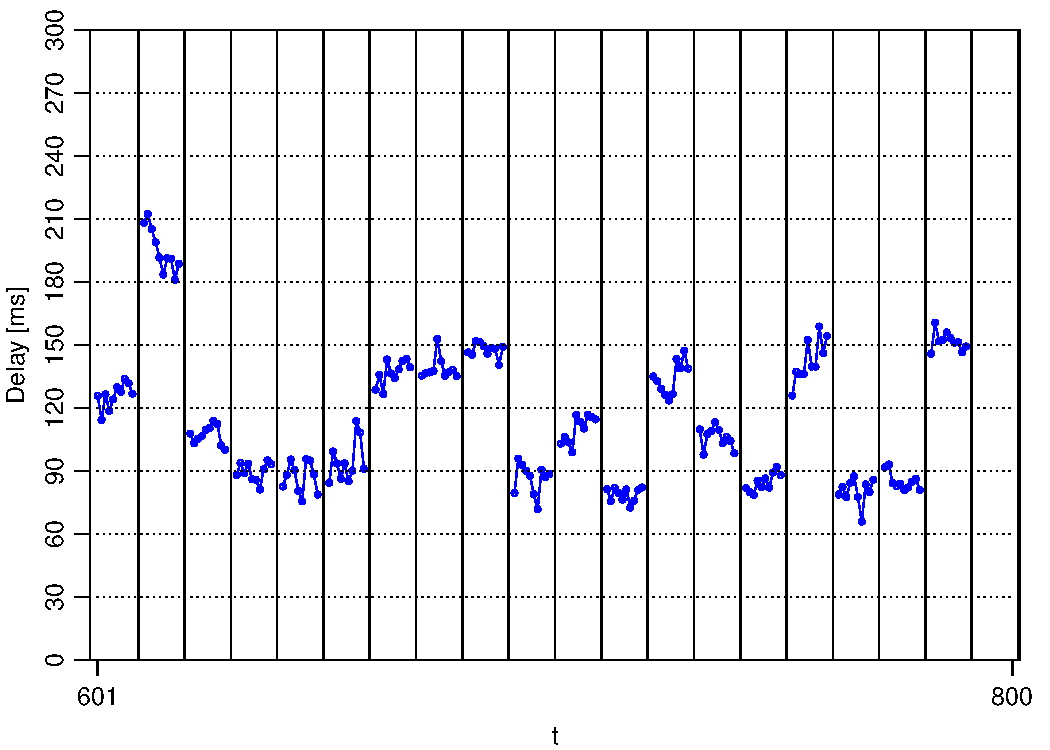
\includegraphics[width=0.4\hsize]{C:/master/mstudy/analysis/FTP/10msFTP/day2/exam1-day2-4th.pdf}
}
\caption{FTP を併用した 10 ミリ秒間隔の実験(二回目)}
\end{center}
\end{figure}
\begin{figure}[tb]
\begin{center}
\subfigure[直後,インデックス 1 から 200 まで]{
\includegraphics[width=0.4\hsize]{C:/master/mstudy/analysis/FTP/10msFTP/day2/exam1-day2-after-1st.pdf}
}~
\subfigure[直後,インデックス 201 から 400 まで]{
\includegraphics[width=0.4\hsize]{C:/master/mstudy/analysis/FTP/10msFTP/day2/exam1-day2-after-2nd.pdf}
}\\
\subfigure[直後,インデックス 401 から 600 まで]{
\includegraphics[width=0.4\hsize]{C:/master/mstudy/analysis/FTP/10msFTP/day2/exam1-day2-after-3rd.pdf}
}~
\subfigure[直後,インデックス 601 から 800 まで]{
\includegraphics[width=0.4\hsize]{C:/master/mstudy/analysis/FTP/10msFTP/day2/exam1-day2-after-4th.pdf}
}\\
\subfigure[別日,インデックス 1 から 200 まで]{
\includegraphics[width=0.4\hsize]{C:/master/mstudy/analysis/FTP/10msFTP/day2/exam1-day2-other-1st.pdf}
}~
\subfigure[別日,インデックス 201 から 400 まで]{
\includegraphics[width=0.4\hsize]{C:/master/mstudy/analysis/FTP/10msFTP/day2/exam1-day2-other-2nd.pdf}
}\\
\subfigure[別日,インデックス 401 から 600 まで]{
\includegraphics[width=0.4\hsize]{C:/master/mstudy/analysis/FTP/10msFTP/day2/exam1-day2-other-3rd.pdf}
}~
\subfigure[別日,インデックス 601 から 800 まで]{
\includegraphics[width=0.4\hsize]{C:/master/mstudy/analysis/FTP/10msFTP/day2/exam1-day2-other-4th.pdf}
}
\caption{FTP を併用した 10 ミリ秒間隔の実験(二回目)}
\label{10ms-2}
\end{center}
\end{figure}

図より,FTP を併用した場合には右下がりの傾向が見て取れない.
また,小さな応答遅延の分布帯は 15 秒間隔での計測と同程度の 60 ミリ秒程度であり,他の 30 ミリ秒程度と比べて大きくなっていた.
理由としては先と同様,FTP 通信を行うために通信リソースが割かれ ICMP パケットの処理が後回しにされているのではないかと考えられる.
以上より,FTP 通信を併用することで 10 回ごとの最初の ping 計測から小さな応答遅延が得られるのではないかという仮説は外れていた.
結果としては一回目の応答遅延を含め,10 回すべての応答遅延が比較的大きな値をとり,そこには減少傾向は見られないようだ.
\end{document}